\definecolor{lightergray}{RGB}{247,247,247}
\definecolor{darkgreen}{RGB}{36,135,20}
\definecolor{green_comment}{RGB}{0,128,0}
\definecolor{redcell}{RGB}{238,176,176}
\definecolor{greencell}{RGB}{217,234,211}


\chapter{Diseño e Implementación de estrategias para aumentar el rendimiento de algoritmos de IA}
\label{cap:c3_implementaciones}	


	
	En este capítulo se presentan los diseños e implementaciones desarrollados a lo largo del trabajo. Inicialmente se presenta una introducción a la liberia MPI, mejorando programas sencillos fuera del ámbito de la inteligencia artificial. Posteriormente, se desarrollan los algoritmos de IA, empezando por los más sencillos y terminando por los más complejos.

%\newpage %TODO QUITAR
\section{Programas sencillos}

	Para introducir MPI en el proyecto se implementan y comentan varios programas sencillos. Primero la multiplicación de matrices, que tiene un coste cúbico O(\(N^{3}\)), al tener que recorrer, para cada elemento de la matriz, una fila y columna entera. Segundo, algoritmos de ordenación, que para simplificar, solo se realiza un estudio de las ordenaciones que más tiempo de ejecución consumen, O(\(N^{2}\)) y MergeSort con coste O(N*logN).


	Las matrices son un concepto matemático muy relevante en el mundo de los videojuegos y en el ámbito de la inteligencia artificial. Hay muchas técnicas de IA que conllevan la gestión de imágenes, como en el algoritmo DQN cuya red neuronal tiene como entrada varios fotogramas para poder aprender. Estas imágenes, pueden en mayor o menor medida ser implementadas con matrices.
	
	El cálculo de la multiplicación de dos matrices es cúbico O(\(N^{3}\)). Ensencialmente, es necesario recorrer toda la matriz, y para cada elemento, realizar el sumatorio de las multiplicaciones fila, columna. 
	
	Por ello, es un buen primer ejemplo para presentar una estrategia basada en MPI, debido al alto coste computacional. Para ello hay que plantear cómo dividir el trabajo entre los procesos. 
	
	Inicialmente, se puede pensar que es mejor enviar los datos conforme se finaliza una operación, pero en esta operación se necesitan las filas de una matriz y columnas de otra, por lo que conviene que cada proceso tenga una matriz entera en su memoria local para agilizar el proceso y poder enviar más datos al mismo tiempo.


	Cada \textit{worker} se va a encargar de un determinado número de filas, paralelizando así el cálculo. El \textit{master} se encarga de dividir la matriz entre los procesos, y se puede abordar con dos enfoques distintos.
	\begin{itemize}
		\item Reparto estático: Los datos se dividen antes de empezar el cálculo. 
		\item Reparto dinámico: Los datos se reparten en tiempo de ejecución, asignando lso mismos de forma proporcional a la velocidad de cada proceso.
	\end{itemize}



	\begin{figure}[!h]
		\centering
		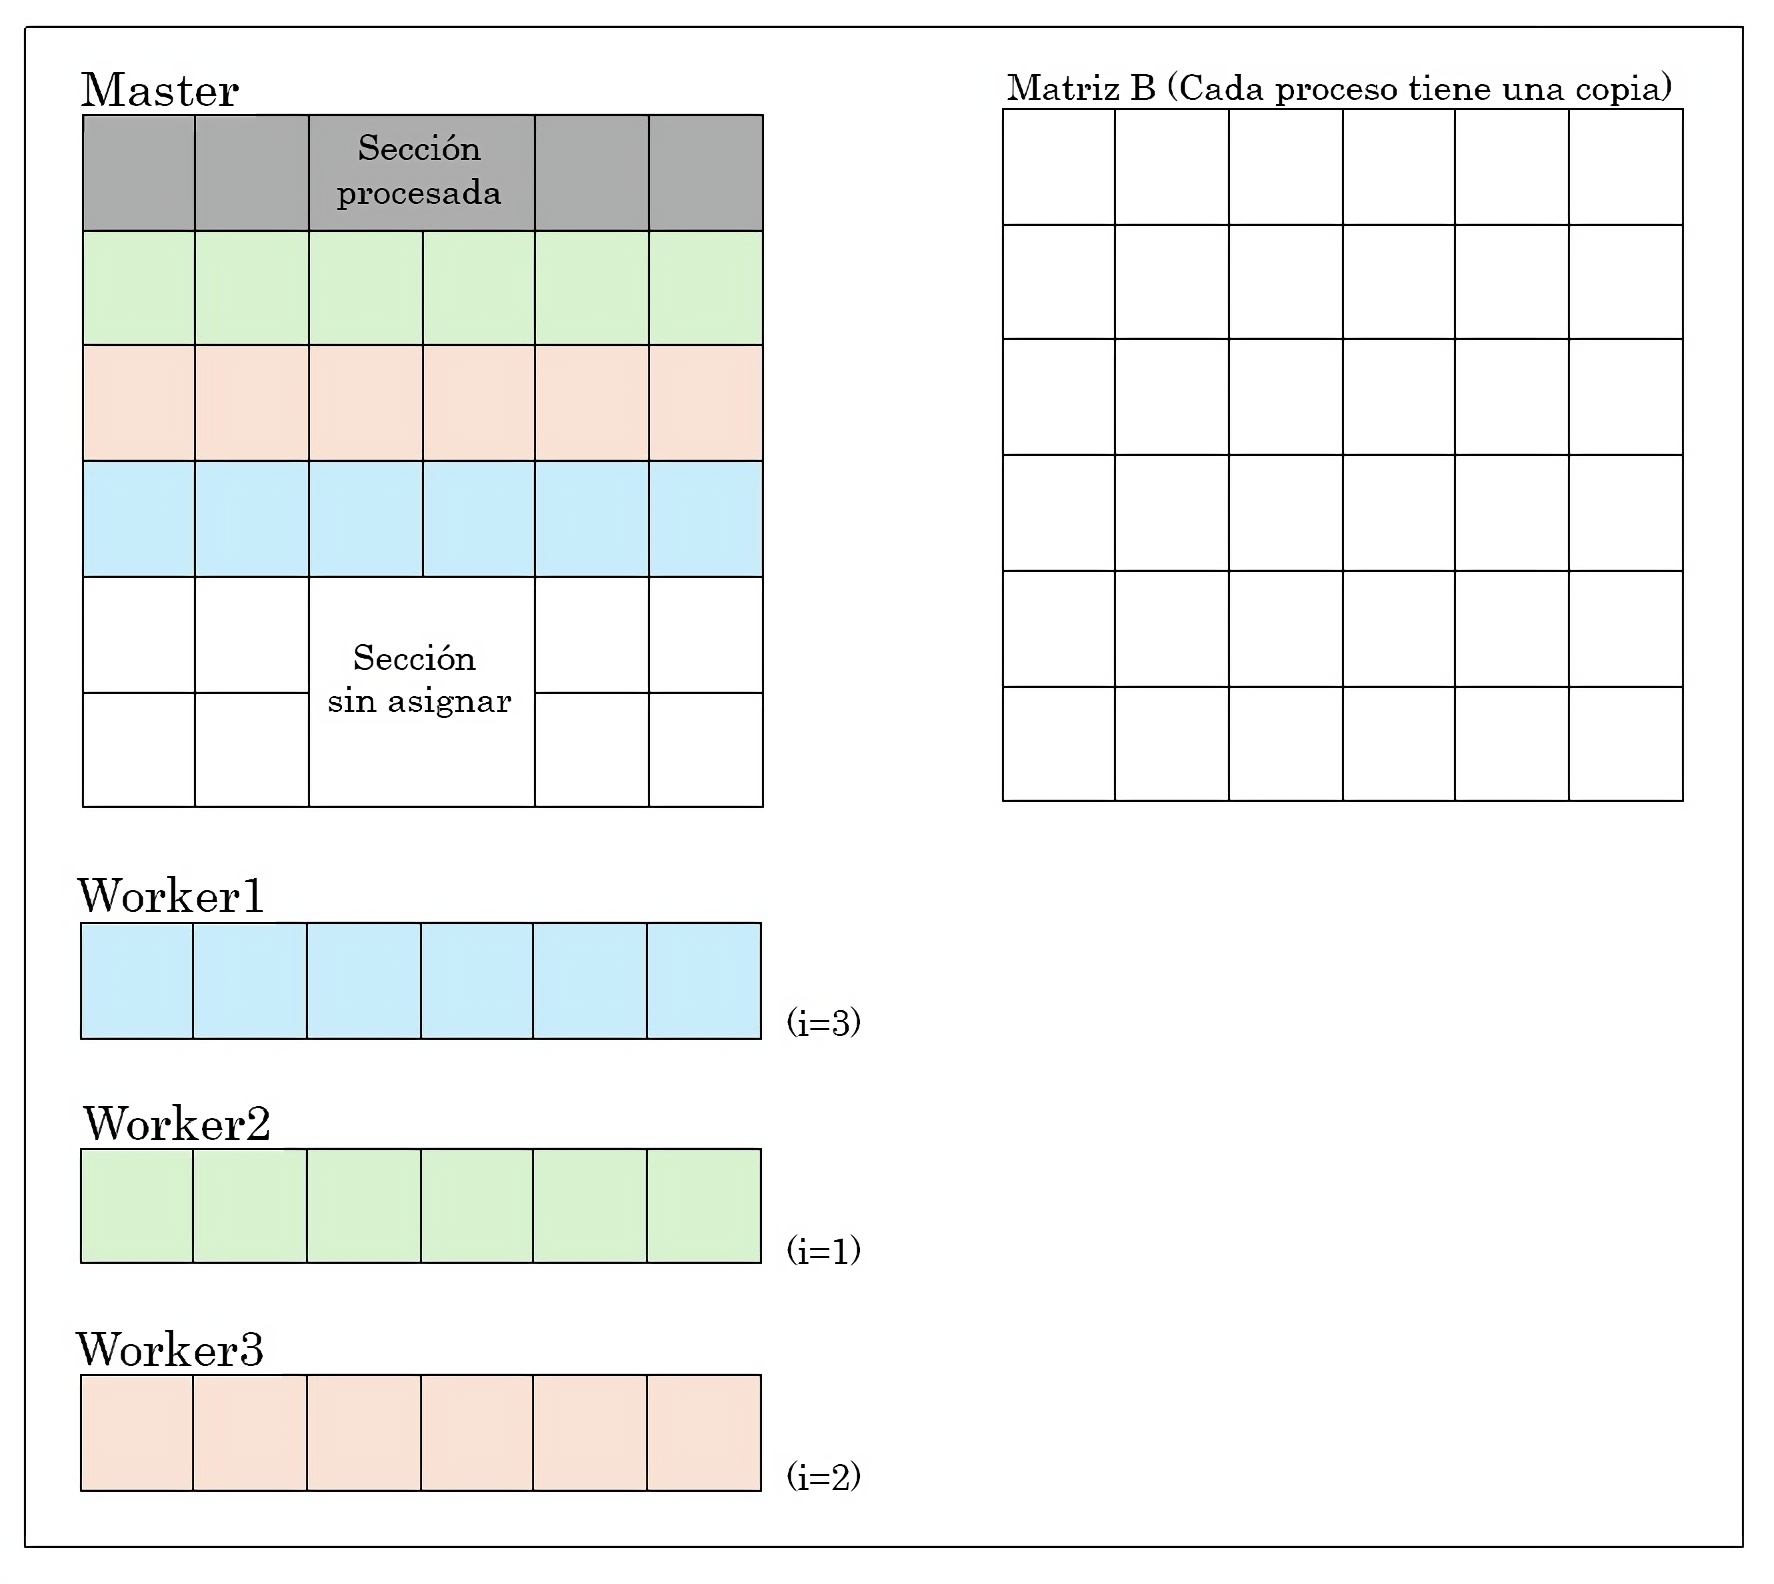
\includegraphics[width=0.58\textwidth]{images/chapter_3/matriz_mpi}
		\caption{MPI - División de datos (ejemplo de multiplicación de matrices)}
		\label{fig:matrizmpi}
	\end{figure}
	
	En la primera estrategia, dividimos la matriz entre todos los \textit{workers}, dejando al \textit{master} en espera de recibir datos. Esta mejora depende de la velocidad de los procesos, pues se puede generar un cuello de botella si todos terminan y envían los datos al mismo tiempo. Además de aumentar la complejidad espacial entre los procesos, pues se divide la matriz entera entre los \textit{workers}. 
	
	En la segunda estrategia, hay un flujo constante de nuevos datos y resultados obtenidos, reduciendo el tiempo perdido en un posible cuello de botella. En la Figura \ref{fig:matrizmpi} se muestra como el \textit{master} divide la matriz, marcando en negro la parte ya procesada. A su vez cada \textit{worker} tiene una sola fila en su memoria, reduciendo la complejidad espacial.
	
	 


	%\vspace*{0.2cm}
	
	
	Los algoritmos de ordenación tienen que iterar varias veces hasta que el array de elementos esté completamente ordenado. Y los métodos pueden variar considerablemente el tiempo de ejecución.
	
	Para las ordenaciones cuadráticas, los métodos populares como BubbleSort, InsertionSort y SelectionSort, han sido estudiados y optimizados para que, aunque tengan un coste cuadrático O(\(N^{2}\)), en el caso peor, proporcionen un buen rendimiento. Basándose en estos algoritmos, se ha diseñado uno adicional llamado SequentialSort. Este algoritmo recorre todas las posiciones del array, y para cada elemento compara todos los datos, sumando en un contador los elementos mayores que el, para calcular así su posición en el array ordenado. Una vez finalizada una iteración, se coloca el elemento en el array ordenado, si la posición actual esta ocupada es porque hay una repetición del elemento, y se tiene que colocar en la siguiente celda libre. La Figura \ref{fig:sequentialsortmpi} representa el proceso de ordenación, marcando en gris el elemento que ha de compararse con los demás en la iteración i-ésima.


	\begin{figure}[!h]
		\centering
		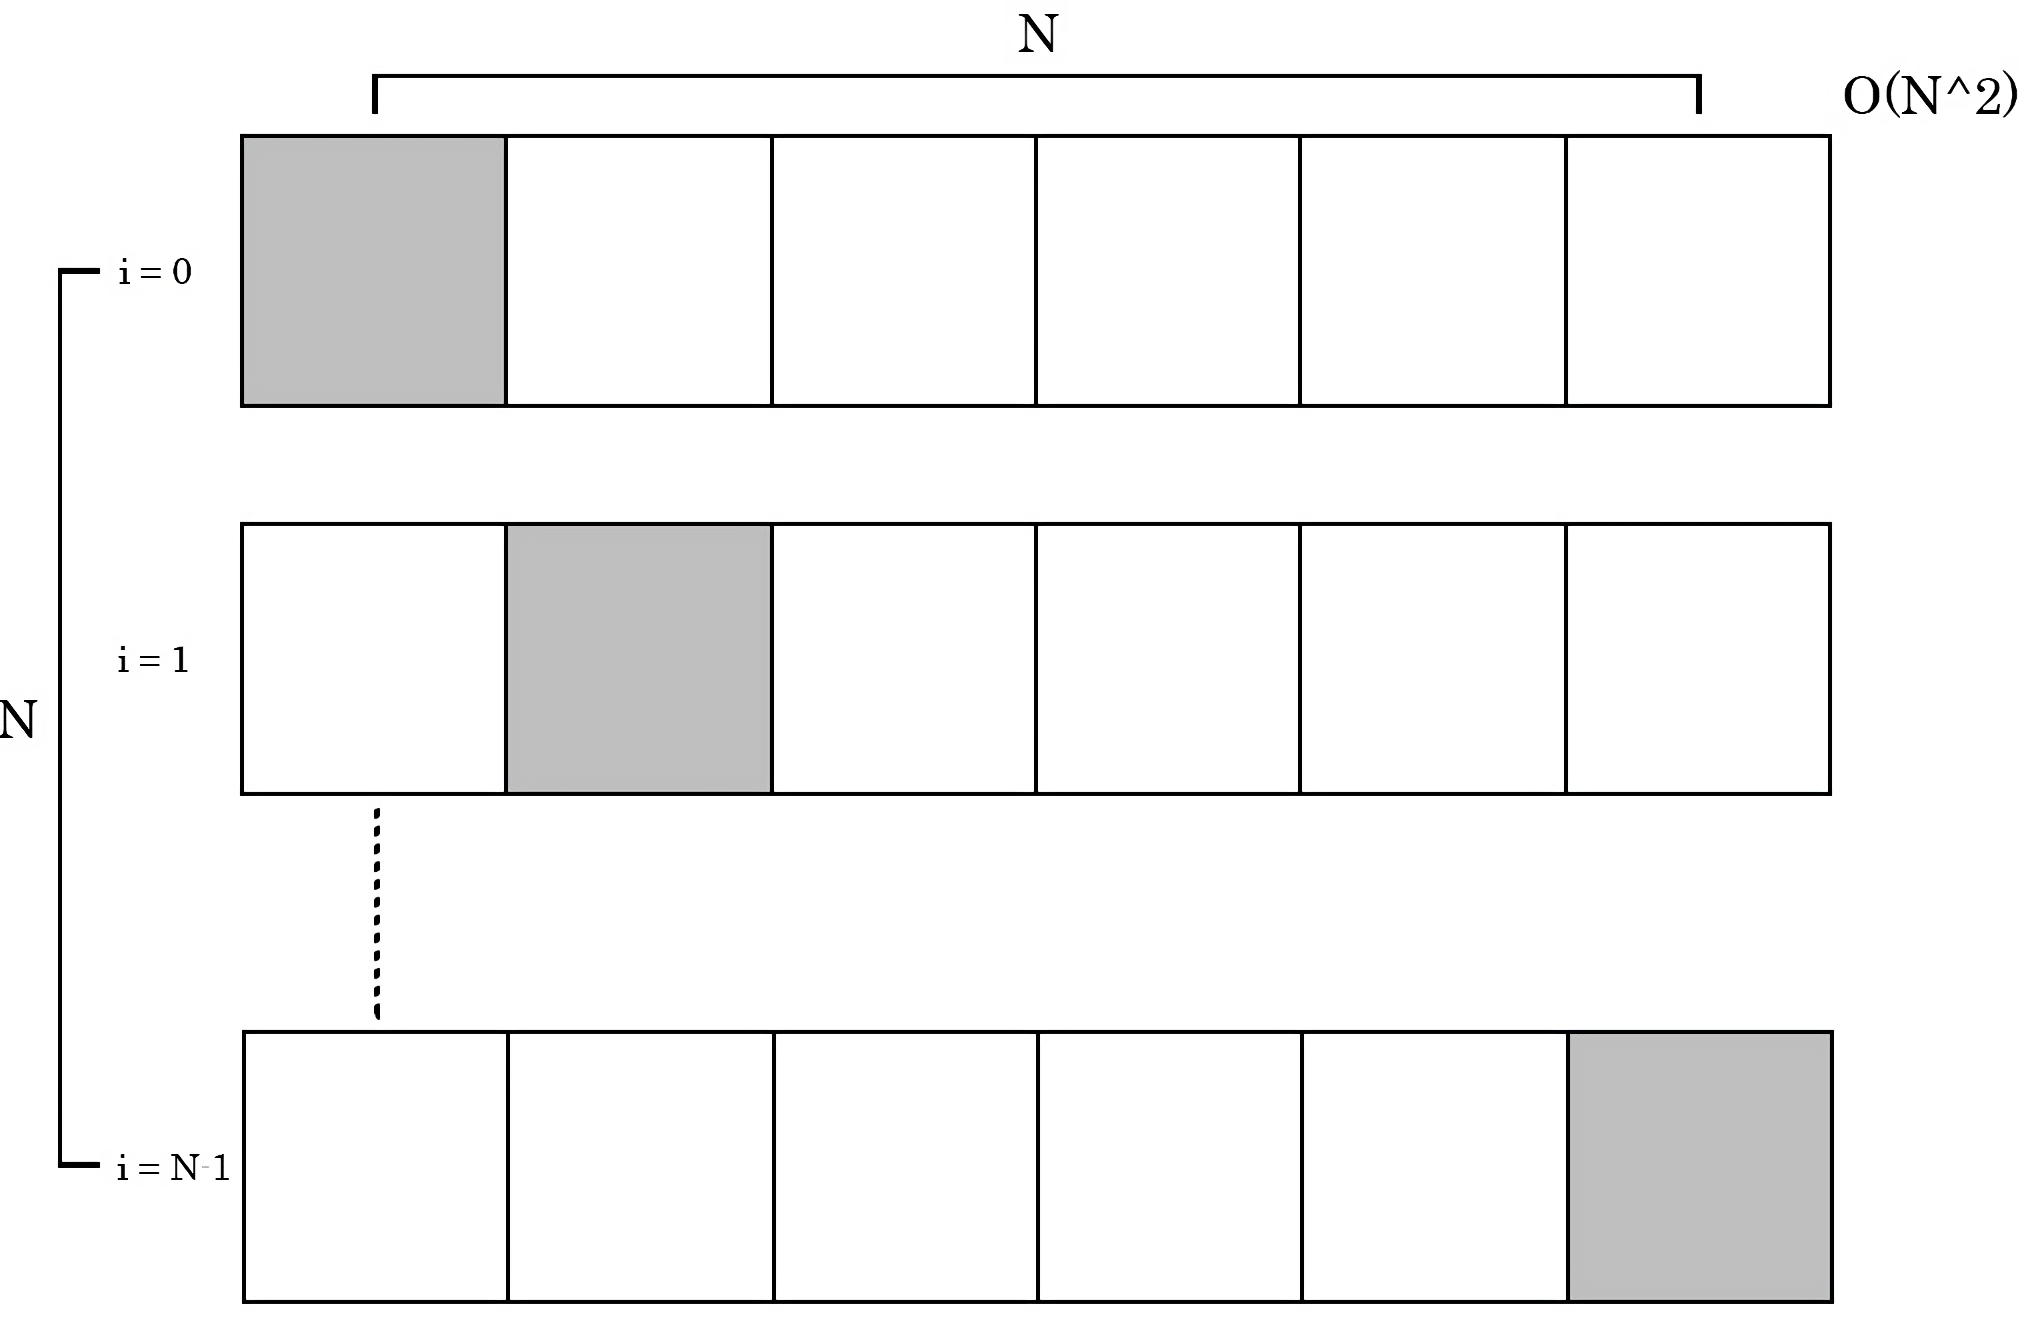
\includegraphics[width=0.6\textwidth]{images/chapter_3/sequentialsort_mpi}
		\caption{MPI - SequentialSort}
		\label{fig:sequentialsortmpi}
	\end{figure}
	
	Este método siempre tendrá coste cuadrático O(\(N^{2}\)). No es como los anteriores que van reduciendo el espacio conforme aumentan las iteraciones, pero es fácilmente paralelizable. 
	
	Para lograr el objetivo, antes de procesar los datos el \textit{master} envía a todos los \textit{workers} el array entero. Una vez recibido el array de elementos, comienza la etapa de enviar y recibir elementos para realizar las comparaciones y enviar las posiciones de los elementos en el array ordenado. 



	Los algoritmos de ordenación logarítmicos son muy útiles y eficientes. QuickSort tiene varios problemas como la profundidad de recursión y en el caso peor es cuadrático. Los algoritmos de RadixSort y HeapSort son eficientes sin aplicar mejoras, y MergeSort es muy popular, tanto que se aplica en Python para el método de ordenación por defecto, TimSort\cite{auger2015merge}. Este último combina InsertionSort, una ordenación cuadrática muy eficiente para ordenar para ordenar pequeños conjuntos de datos, teniendo una baja sobrecarga en términos de operaciones. Para luego usar las mitades ordenadas con MergeSort. Sin embargo, el algoritmo básico de MergeSort no es tan eficiente.
	
	Aplicando la misma idea que TimSort, se puede mejorar el tiempo de ejecución de MergeSort, aplicando combinaciones de los métodos básicos con complejidad cuadrática y comprobar la eficiencia.
	
	
	Aplicando MPI se crean varios procesos (para mayor eficacia y simplicidad, el número de procesos tiene que ser potencia de dos), y se divide el array entre los procesos. Las fase de esta mejora son:
	\begin{itemize}
		\item Primera fase de ordenación: cada proceso ordena su sub-array con el método de ordenación correspondiente. En el capítulo \ref{cap:c4_estudio}, se realiza un estudio de los algoritmos cuadráticos y SelectionSort es el algoritmo que mejores resultados obtiene.
		\item Segunda fase de reagrupación y ordenación: esta fase se repite hasta solo tener un proceso activo, es decir, el array esté completamente ordenado.
	\end{itemize}
	
	En la comunicación entre procesos, cada uno se conecta con el proceso activo más cercano. El proceso de mayor ID (\textit{rank}) envía su array ordenado y finaliza su ejecución. El proceso receptor se encarga de ordenar ambas mitades en una sola. Utilizando una barrera (barrier MPI), garantizamos que todos terminen al mismo tiempo. Esta mejora aplica la idea de sincronización con \textit{barrera simétrica mariposa}. Esta técnica de sincronización conecta los procesos dos a dos, aumentando la distancia de los procesos para que en aproximadamente M iteraciones (\(2^{M}\) = número de procesos), todos los procesos estén sincronizados. Para la mejora implementada, se sincronizan por orden de cercanía entre IDs. La Figura \ref{fig:mergesortmpi} muestra el proceso de sincronización, en cada iteración se finaliza la ejecución de los procesos en rojo.  
	
	\vspace{0.2cm}
	
	\begin{figure}[!h]
		\centering
		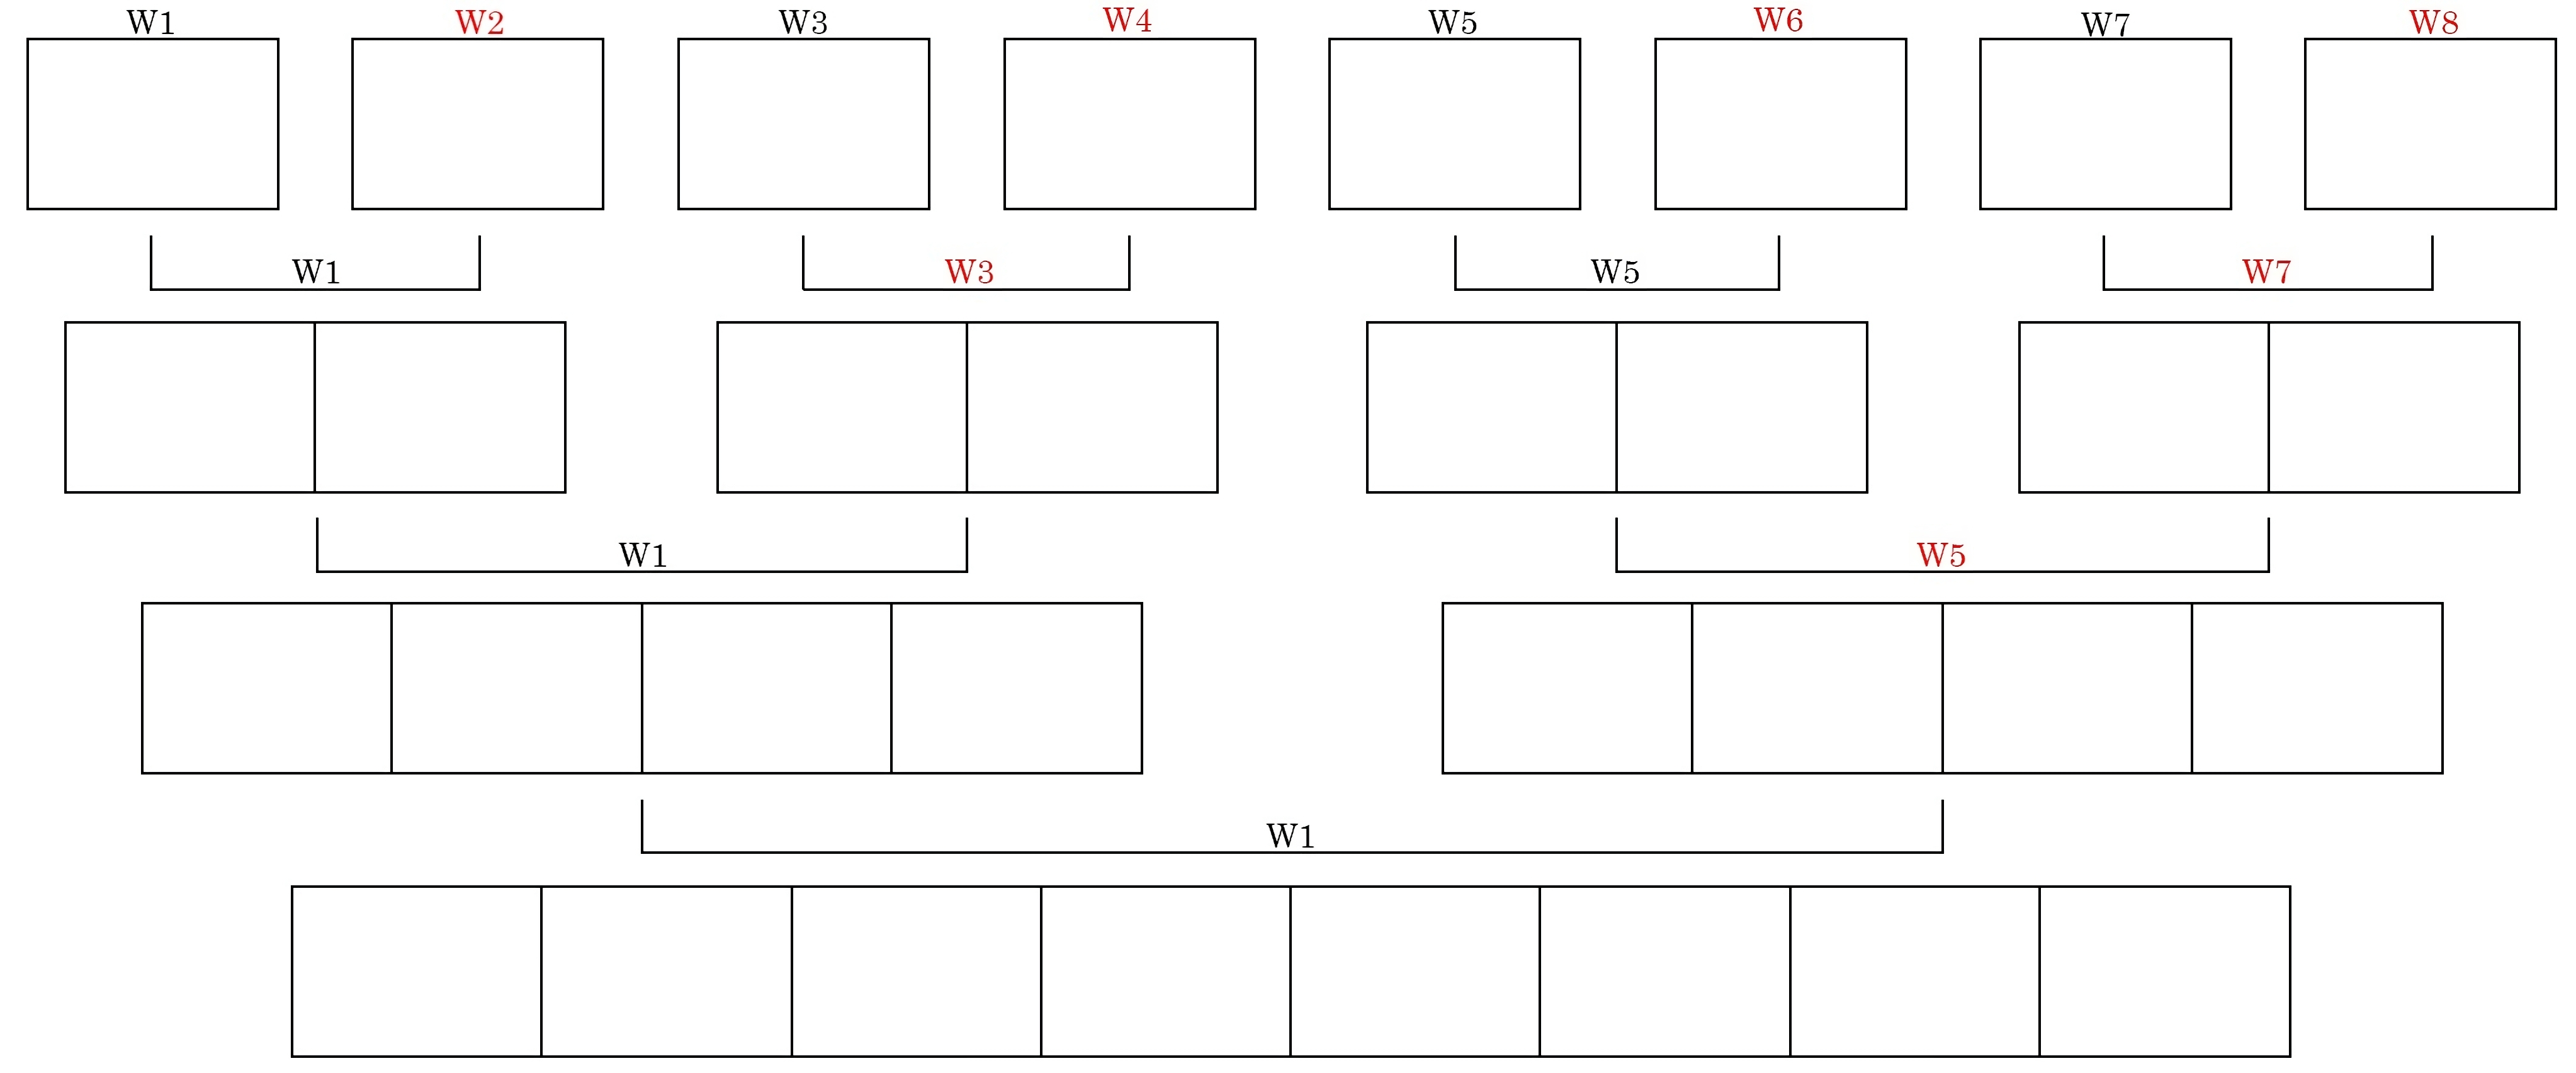
\includegraphics[width=0.85\textwidth]{images/chapter_3/mergesort_mpi}
		\caption{MPI - MergeSort con 8 procesos worker \(W_{1}\) ... \(W_{8}\)}
		\label{fig:mergesortmpi}
	\end{figure}

	%\begin{figure}[!h]
	%	\centering
	%	
	%	
	%	\begin{subfigure}[t]{0.33\textwidth}
	%		\centering
	%		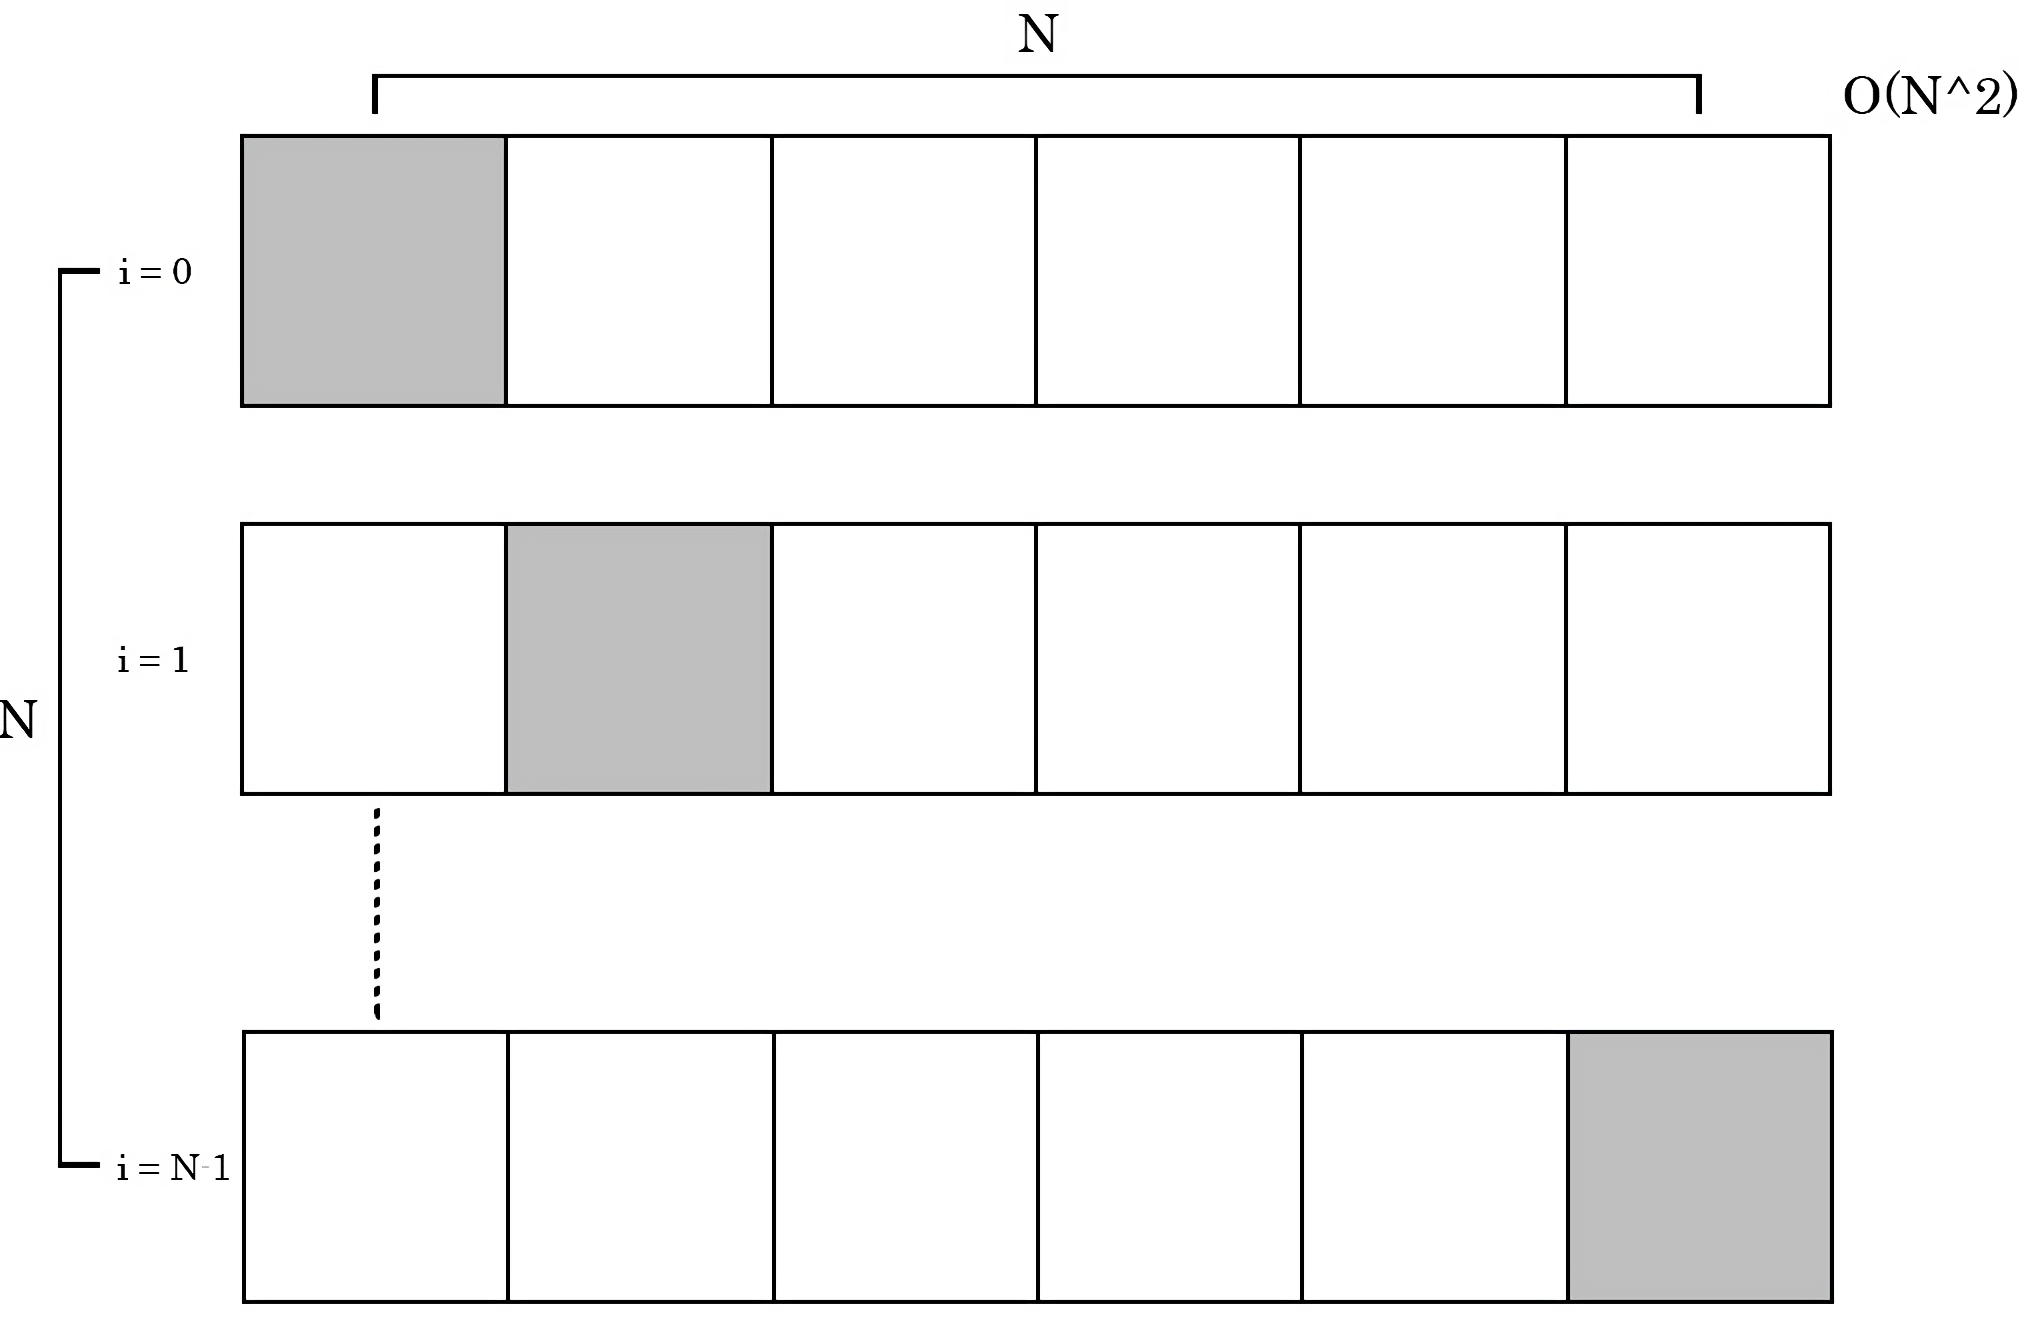
\includegraphics[width=\textwidth]{images/chapter_3/sequentialsort_mpi}
	%		\caption{MPI - SequentialSort}
	%		\label{fig:sequentialsortmpi}
	%	\end{subfigure}
	%	\hfill
	%	\begin{subfigure}[t]{0.48\textwidth}
	%		\centering
	%		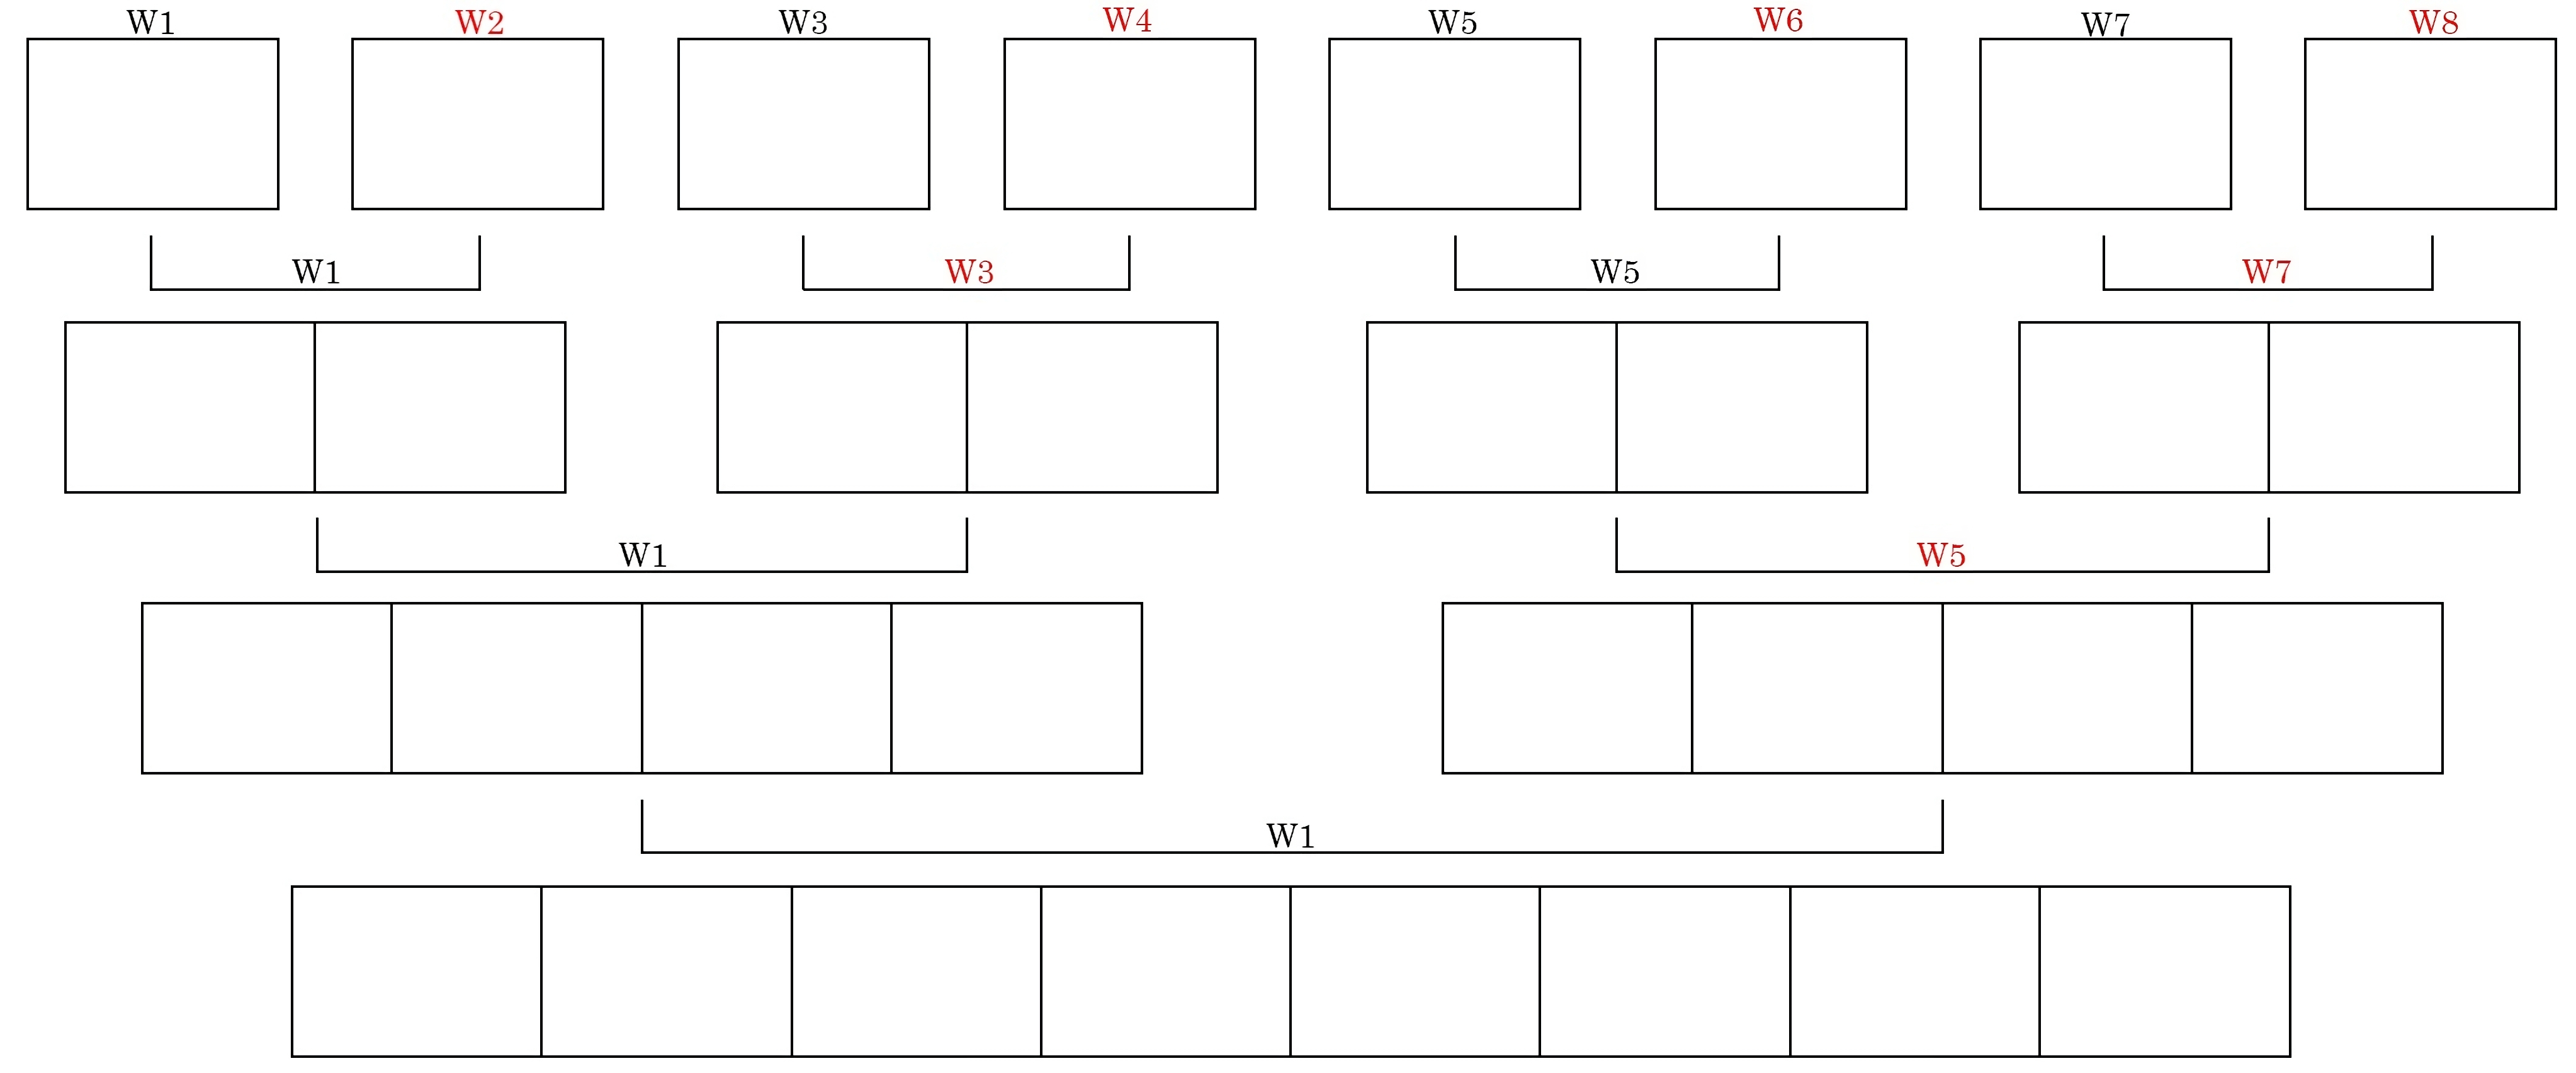
\includegraphics[width=\textwidth]{images/chapter_3/mergesort_mpi}
	%		\caption{MPI - MergeSort}
	%		\label{fig:mergesortmpi}
	%	\end{subfigure}
	%	
	%	\caption{Mejoras MPI de las ordenaciones}
	%	\label{fig:ordenacionesmpi}
	%\end{figure}

	
	Para aplicar MPI y paralelizar programas hay que tener en cuenta que la comunicación entre procesos requiere un tiempo para enviar/recibir mensajes. Si queremos reducir el tiempo de ejecución de un programa tenemos que asegurarnos que la estrategia es viable para mejorar el rendimiento. Si ejecutamos, por ejemplo, una búsqueda lineal en un array, a primera vista, reducir el espacio de búsqueda puede ser beneficioso. Dividiendo el espacio de búsqueda entre los \textit{workers} reduce el tiempo de O(N) a O(N/numWorkers). Pero ¿se puede reducir el tiempo de ejecución al dividir el espacio entre los \textit{workers}? 
	
	Para responder esta pregunta es necesario tener en cuenta el tiempo de paso de mensajes (overhead). Si no se tuviese en cuenta, se podría garantizar la reducción, pero la comunicación entre procesos tiene un coste, y con un tiempo lineal, generalmente no se pueden lograr mejoras, más bien aumenta el tiempo de búsqueda.
	
	Por este motivo, hay que tener en cuenta la complejidad temporal de los algoritmos que queremos optimizar, ya que no siempre es eficiente aplicar paralelismo.

	\newpage 

\section{Algoritmos de Clustering}

	Una vez introducido MPI con programas básicos, podemos presentar las implementaciones de los algoritmos relacionados con la inteligencia artificial. Las técnicas de clustering toman una población y, dependiendo del conjunto de datos, categoriza los individuos. Los algoritmos pueden ser supervisados, si ademas de la población a categorizar, tenemos un poblacion categorizada previamente, o no-supervisados, si no contamos con esta población etiquetada.

	\subsection{Jerárquico Aglomerativo}
		Este algoritmo usa una matriz para calcular las agrupaciones. Como es una matriz simétrica, podemos reducir la complejidad espacial usando solo el triángulo superior. 
		
		La distancia entre clusters es muy importante. Además de calcular agrupaciones distintas, también varía la complejidad temporal. La más eficaz y rápida es la de centroides. Para calcular la distancia entre dos cluster solo necesita el cálculo entre dos puntos (los centros de los clusters). 
		
		El calculo de la distancia por enlace simple y completo, es más complejo. Cada cluster almacena las coordenadas de sus individuos, para, a la hora de calcular la distancia entre dos clusters (\(C_{i}\) y \(C_{j}\)), comprobar la distancia de cada par de puntos (donde uno pertenece a \(C_{i}\) y el otro a \(C_{j}\)). La nueva distancia usando enlace simple es la mínima distancia entre cualquier par de puntos, mientras que la completa es la máxima distancia.
		
	
		Una vez implementadas las mejoras en el cálculo de multiplicación de matrices, podemos usar estas para mejorar este algoritmo. La primera idea de enviar las filas conforme se realizan los cálculos no se puede aplicar. El algoritmo es más complejo que realizar sumatorios de multiplicaciones (suma de productos, para la multiplicación de matrices), pues la matriz está en constante cambio. Tendría que realizarse un proceso de comunicación costante para gestionar la matriz. Esto y añadir más operaciones del algoritmo para agrupar los individuos, provoca que no sea viable realizar esta mejora. Si dividimos la matriz entre los \textit{workers} cada proceso se encarga de una zona y paralelizamos así el trabajo a realizar.
		
				
		Como es una matriz simétrica y se representa con el triángulo superior, hay que dividir la carga de trabajo equitativamente. No podemos implementar una mejora sin dividir el espacio de forma óptima entre los \textit{workers}. Si dividimos las filas de forma secuencial, el primer \textit{worker} tendrá muchos más elementos que el último, parando la ejecución por ``culpa'' del primer proceso. La Figura \ref{fig:prueba} muestra el cálculo de elementos a procesar entre el primer y último \textit{worker} si no se divide el espacio de manera óptima. 
		
		
		
		\begin{figure}[!h]		
		\begin{mdframed}[roundcorner=5pt]
			\[
			\sum_{i=1}^{\text{filas}} (N - i) \gg \sum_{i=\text{filas}(M-1)}^{\text{filas}(M-1) + \text{filas}} (N - i)
			\]
			\begin{tcolorbox}[boxrule=0.5pt, fontupper=\small]
				
				\textit{N} individuos de la población, \textit{M} procesadores. \textit{N/M} filas para cada worker.\\
				
				Con 100 individuos de población y 4 workers, cada uno tendrá 25 filas. Por lo que:
				\begin{itemize}
					\item \(W_{1}\) tiene las filas de 1-25, con 2175 elementos. 
					\item \(W_{4}\), las filas de 76-100, con solo 300 elementos. 					
				\end{itemize}
				
				\(W_{1}\) tiene 7.25 veces más elementos, no se reducirá el tiempo de ejecución.
				
							
			\end{tcolorbox}
			
		\end{mdframed}
		
		\caption{Jerárquico Aglomerativo - Cálculo de elementos a procesar usando una distribución secuencial de filas}
		\label{fig:prueba}
		\end{figure}
		
		
		Dividiendo las filas por pares (parte superior, parte inferior) conseguimos una distribución mucho más eficiente. La Figura \ref{fig:aglomerativo} muestra como se distribuyen las filas en cada worker. Así cada \textit{worker} tiene aproximadamente el mismo número de elementos que calcular y analizar, inicialmente. Puede variar si el número de filas no es divisible entre en número de procesos \textit{workers} 
		
		\begin{figure}[!h]
			\centering
			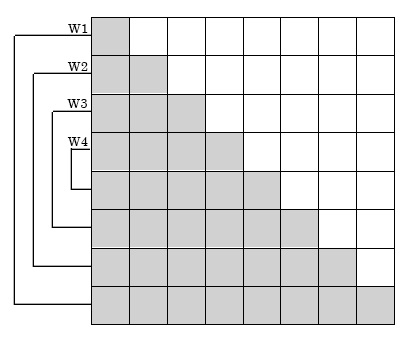
\includegraphics[width=0.55\textwidth]{images/chapter_3/aglomerativo_mpi}
			
			
			\caption{Jerarquico Aglomerativo - División de las filas}
			\label{fig:aglomerativo}
		\end{figure}
		
		%\begin{figure}[!h]
		%	\centering
		%	
		%	
		%	\begin{subfigure}[t]{0.4\textwidth}
		%		\centering
		%		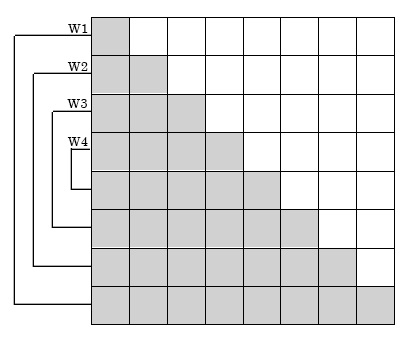
\includegraphics[width=\textwidth]{images/chapter_3/aglomerativo_mpi}
		%		\caption{División óptima}
		%		\label{fig:aglomerativompi}
		%	\end{subfigure}
		%	\hfill
		%	\begin{subfigure}[t]{0.52\textwidth}
		%		\centering
		%		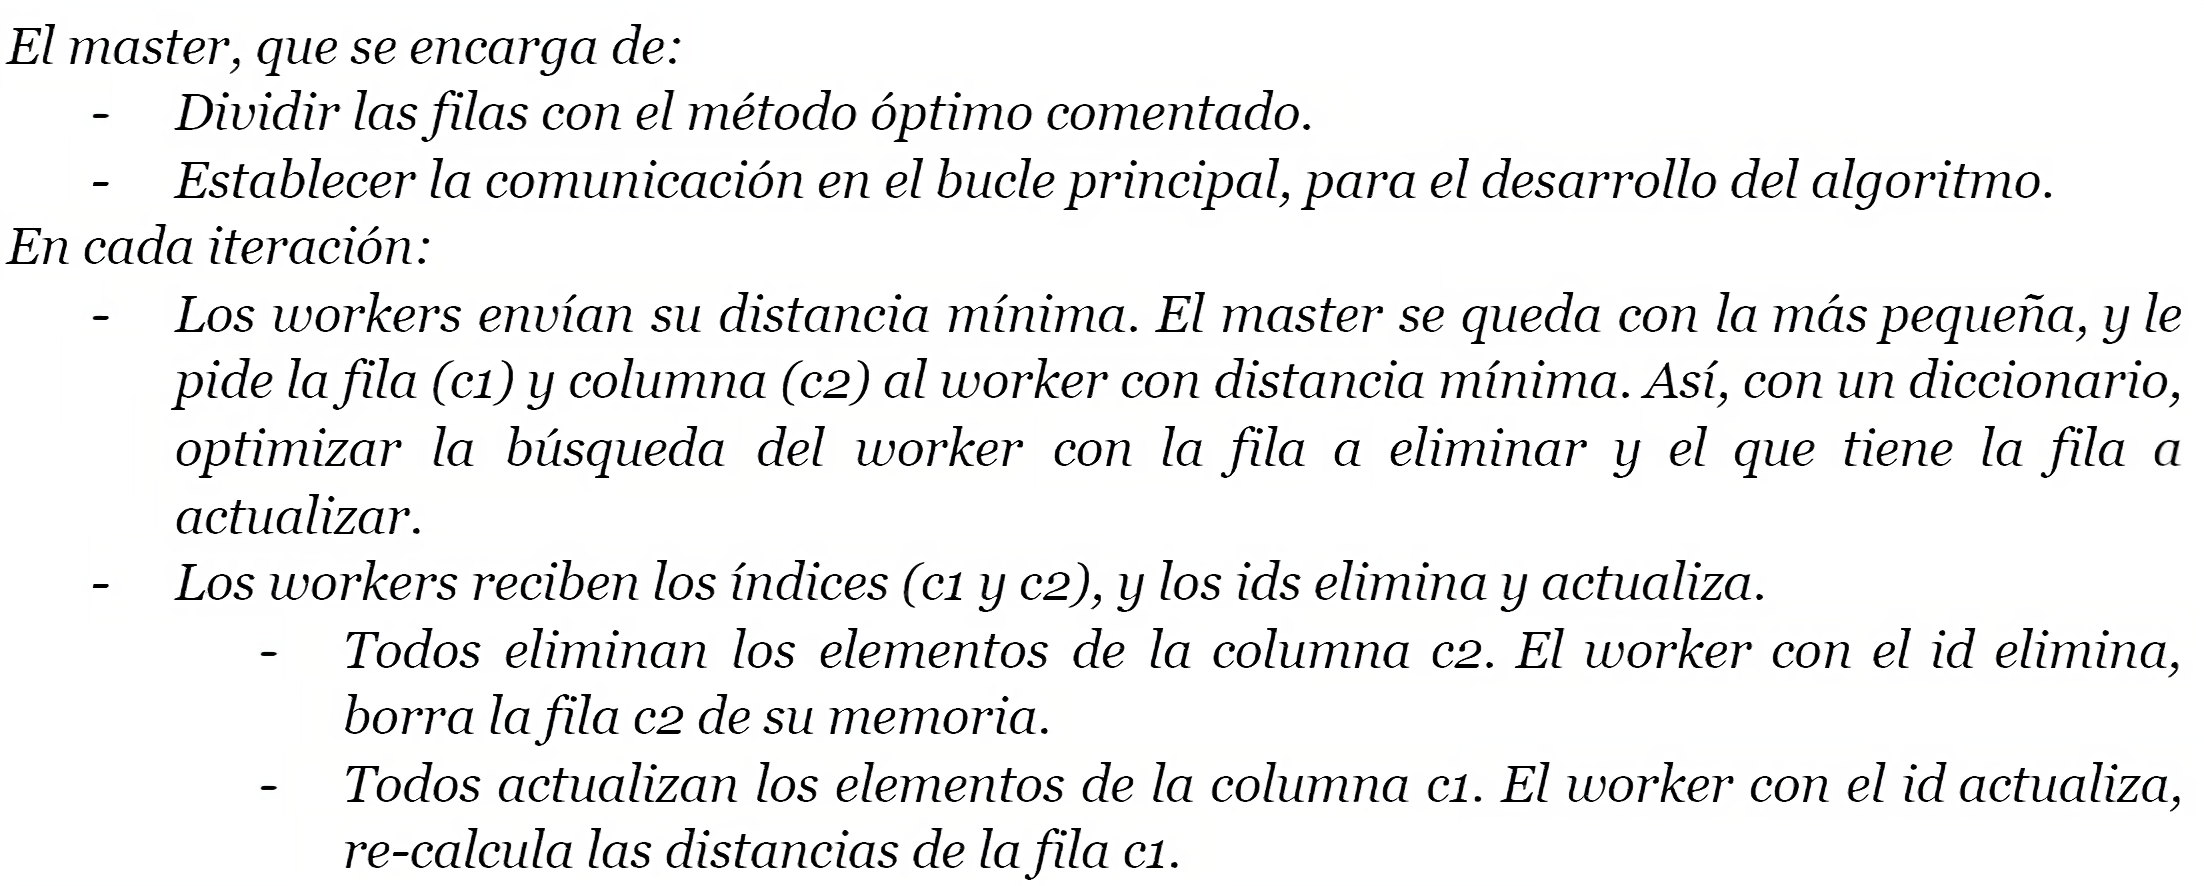
\includegraphics[width=\textwidth,height=5cm]{images/chapter_3/aglomerativo_sec}
		%		\caption{Tareas de los proceso}
		%		\label{fig:aglomerativosec}
		%	\end{subfigure}
		%	
		%	\caption{MPI - Jerarquico Aglomerativo}
		%	\label{fig:aglomerativo}
		%\end{figure}
		
		
		Una vez descrito el reparto de espacio entre los procesos, cada uno tiene que ejecutar el algoritmo en paralelo, sincronizándose cada cierto tiempo para actualizar valores.
		
		Refrescando la memoria, este algoritmo en cada iteración agrupa los dos individuos más cercanos. Eliminando una fila y columna de la matriz.
		
		\newpage
		
			
			
		
		El cálculo de las distancias de la nueva fila usando distancias de centroides es lineal, no se puede reducir el tiempo de ejecución. Pero para los enlaces simples y completos, que tienen un coste cuadrático, se debe intentar reducir el tiempo de cómputo. Para lograrlo se puede dividir el cálculo entre todos los \textit{workers}. 
		
		El objetivo es encontrar una manera lo maás optimizada posible de realizar el cálculo. 
		\begin{itemize}
			\item Cuando hay pocos individuos por \textit{cluster}, es más probable que haya muchas columnas que actualizar, y conviene dividir el cálculo de distancias de todas las celdas entre los procesos disponibles. 
			\item Sin embargo, cuando aumenta el número de individuos, se reducen las columnas y esta idea ya no resulta viable. Cada proceso requiere de un cómputo significativo realizando los cálculos. Por eso, es mejor calcular las distancias de forma escalonada usando todos los \textit{worker}, dividiendo los individuos del \textit{cluster} para encontrar la distancia mínima (simple) o máxima (completa).
		\end{itemize}
		
		Antes de procesar los datos, el \textit{master} divide las filas con el método comentado. 
		
		El siguiente proceso se repite hasta que el solo haya \textit{C clusters}: \color{blue} TODO CREAR UNA FIGURA CON PHOTOSHOP. POR AHORA DEJO EL PROCESO \color{black}
		
		\begin{figure}[!h]
			\centering
			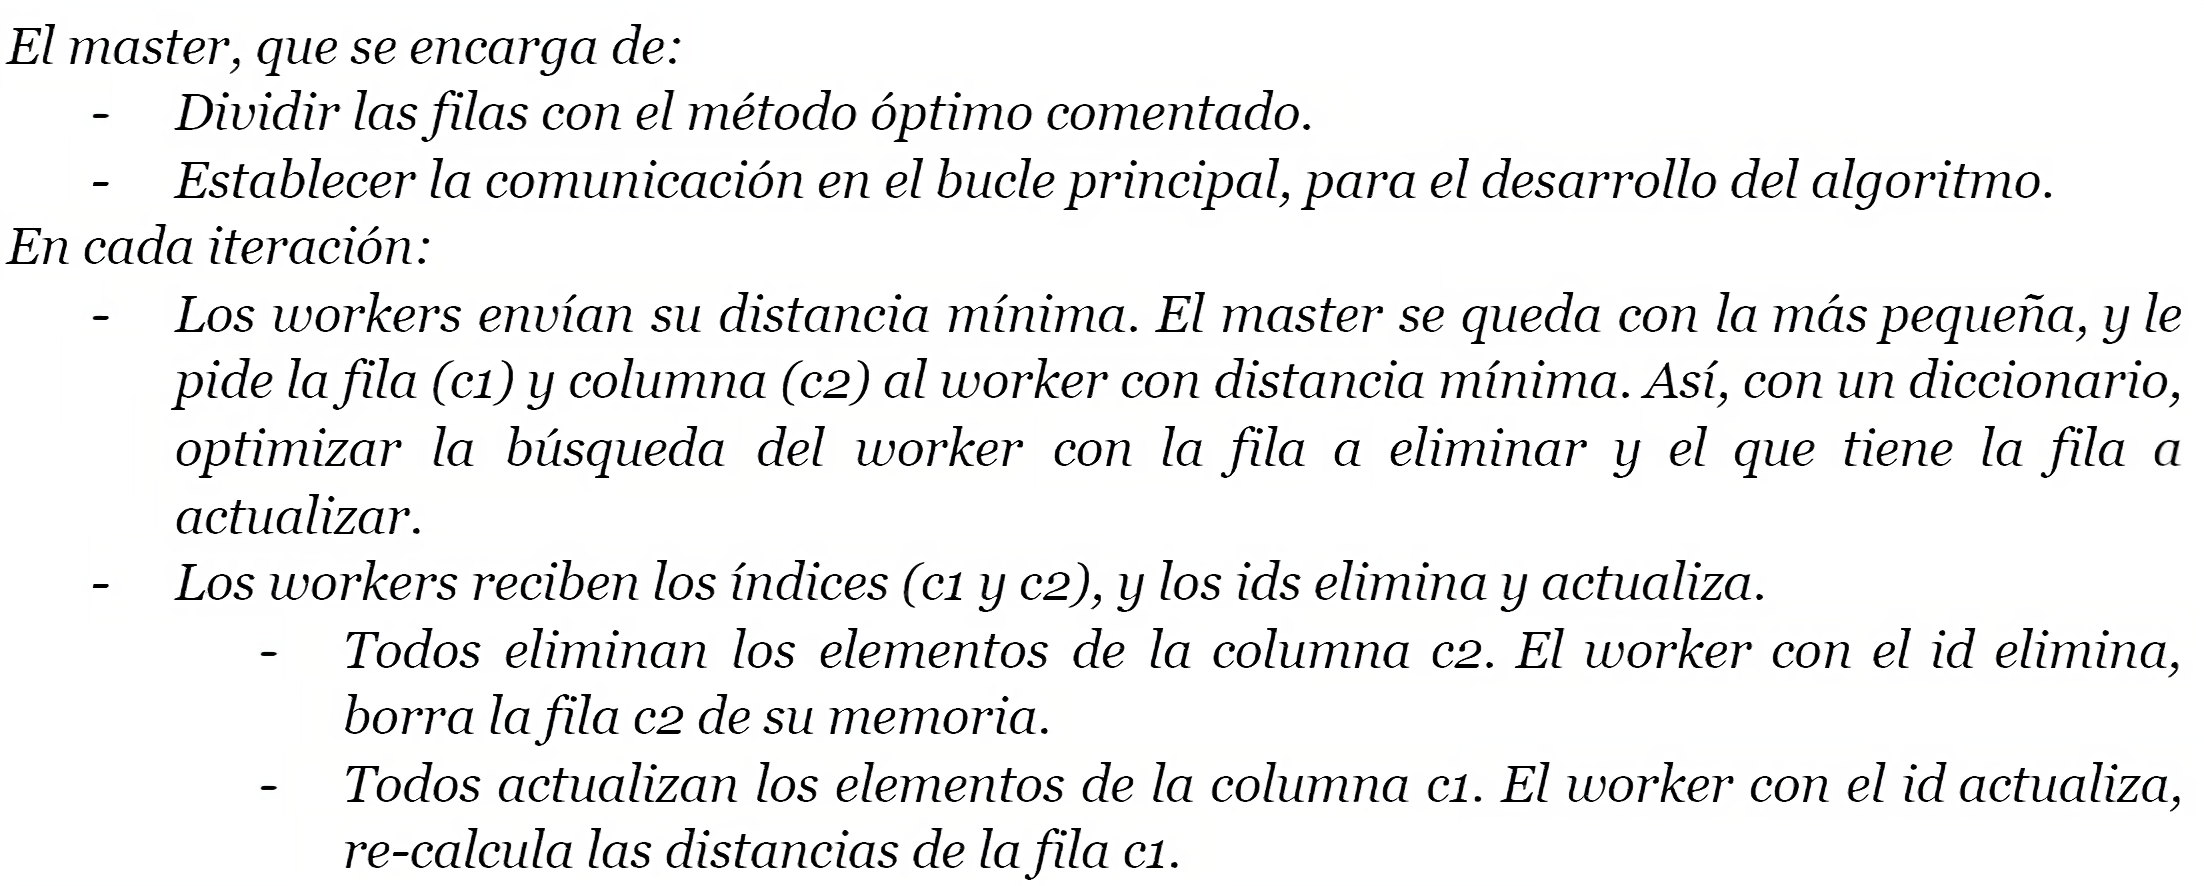
\includegraphics[width=0.65\textwidth]{images/chapter_3/aglomerativo_sec}
			
			
			\caption{Jerarquico Aglomerativo - Proceso de la mejora}
			\label{fig:JA}
		\end{figure}
		
		
		
		
	\subsection{K-Medias}
		Perteneciente al aprendizaje no supervisado, es una técnica de clustering en la cual tenemos una población inicial de individuos sin clasificar, y un valor K sujeto a una asignación flexible según nuestros criterios. Al contrario del algoritmo anterior, no se usa una matriz, y solo se usa distancia por centroides. Una posible mejora puede consistir en las siguientes estrategias:
		
		
		
		\begin{enumerate}
			\item Reparto estático. Dividir la población entre los workers, como muestra la Figura \ref{fig:kmediasdiv}. 
			\item Reparto dinámico. En cada iteración del algoritmo, \textit{master} envia individuos a los \textit{workers}. Cuando finalicen el procesado, envían de vuelta la agrupación y esperen a recibir otros individuos. 
		\end{enumerate}
		
		La primera idea es la más simple y la que mejor suena en un primer momento. El master se encarga de generar los centroides de manera aleatoria, eligiendo K individuos al azar, sin repeticiones. Mediante broadcast los workers reciben estos centros, y con conexiones punto-a-punto se recibe la población dividida sin intersecciones. Cada worker se encarga de una subpoblación. 
		
		
		\color{blue} TODO CREAR UNA FIGURA CON PHOTOSHOP. POR AHORA DEJO EL PROCESO \color{black}
		
		\begin{mdframed}[roundcorner=5pt]
			El siguiente proceso se repite hasta que el \textit{master} envíe un mensaje de finalización, es decir, no cambien los centros:	
			\begin{itemize}
				\setlength\itemsep{0em} % Ajusta el espaciado entre los ítems
				\item Los \textit{workers} calculan la asignación de sus individuos. Además, calculan la suma de distancias de los individuos a sus centros y el número de individuos asociado a cada cluster. Estos valores los envían al \textit{master}.
				\item El \textit{master} recibe estos valores y calcula los nuevos centroides. Manda un mensaje a todos los \textit{workers}. 
				\begin{itemize}
					\setlength\itemsep{0em} % Ajusta el espaciado entre los ítems
					\item \textit{CentroidesNuevos}, si los centros cambian. Se actualizan los centros.
					\item Finalización, en caso contrario.
				\end{itemize}
			\end{itemize}
		\end{mdframed}
		
	
		
		Después de implementar la primera opción, reparto estático, no es una buena idea implementar un reparto dinámico, pues el constante flujo de mensajes aumenta el tiempo de ejecución. La población a categorizar no cambia, por lo que distribuir la población una única vez en toda la ejecución es más eficiente. Lo único que cambia en cada iteración es la asignación de los individuos, pues el algoritmo finaliza cuando la asignación no varíe entre iteraciones (centros de los clusters).
		
		
		\begin{figure} [!h]
			\centering
			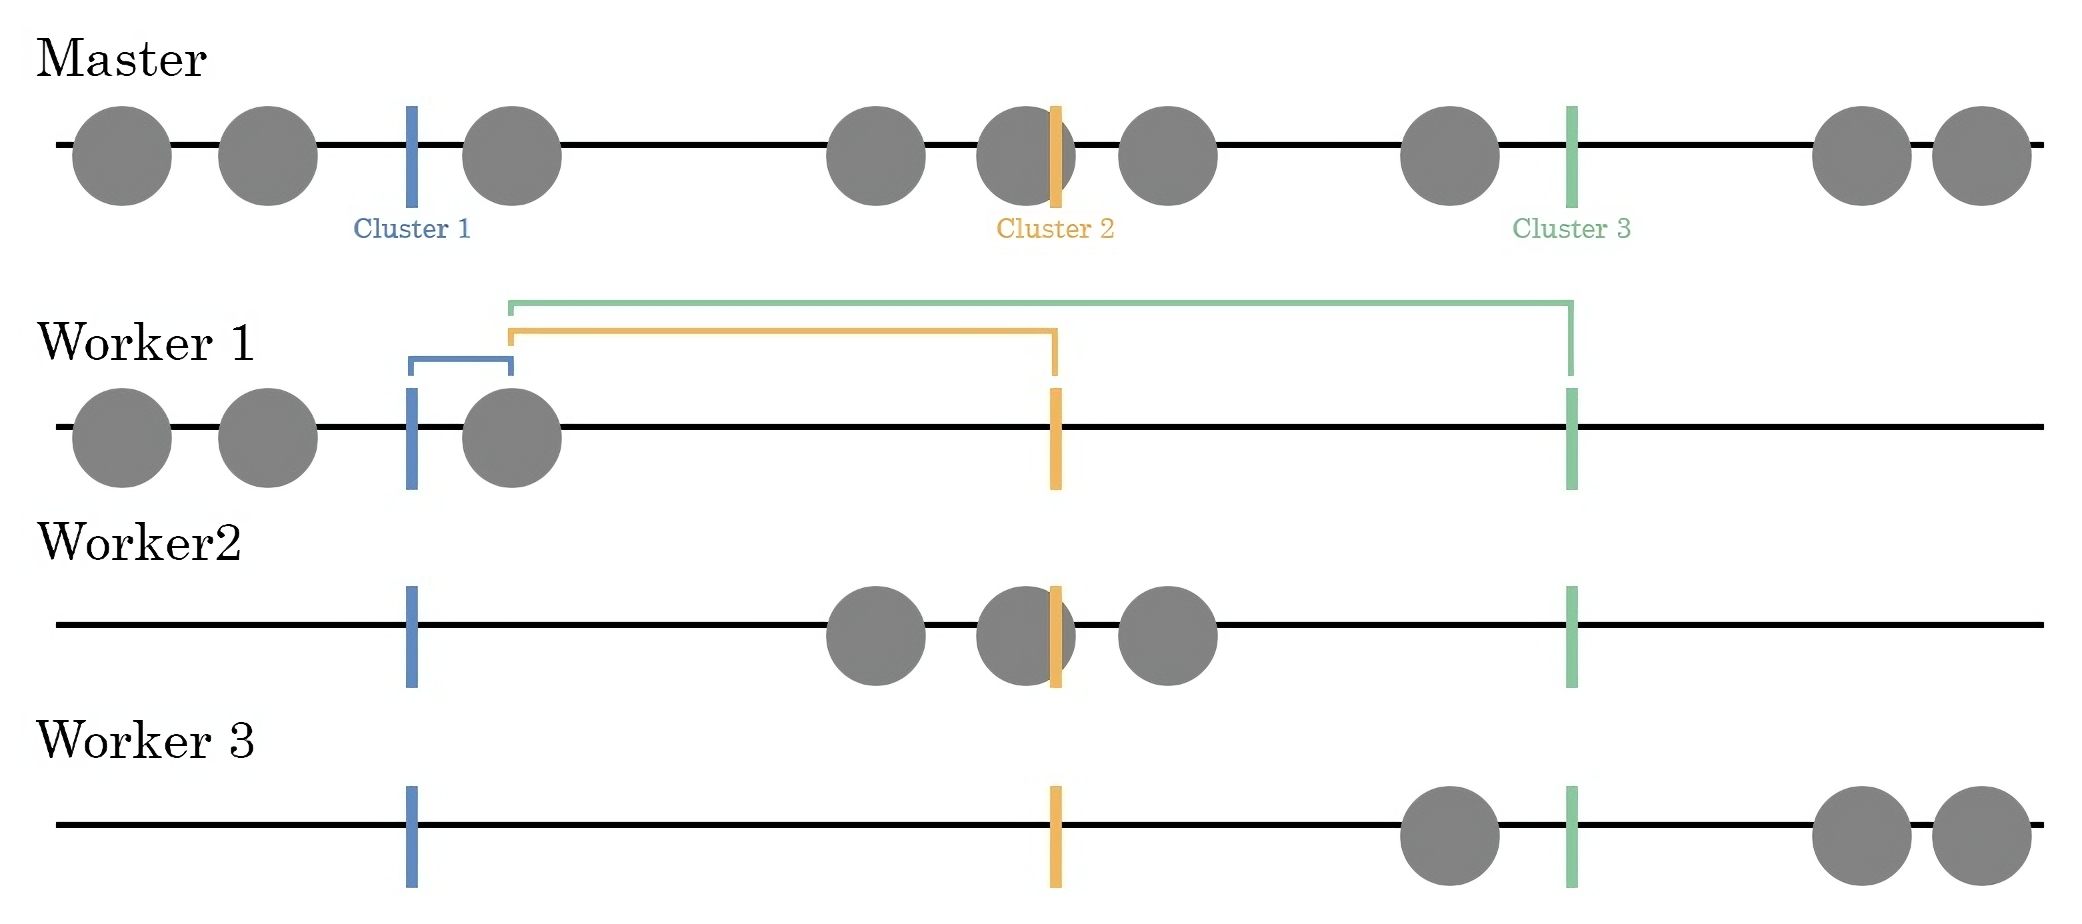
\includegraphics[width=0.8\textwidth]{images/chapter_3/kmedias_mpi}	
			\caption{KMedias - División de poblaciones}
			\label{fig:kmediasdiv}
		\end{figure}
		
		\vspace{0.2cm}
		
		Como se comentó en el capítulo anterior, este algoritmo se tiene que repetir varias veces para encontrar la mejor asignacion, el óptimo general. A su vez, también hay que variar el valor de \textit{K} para buscar la mejor asignación para los individuos. Para lograr este objetivo se puede enfocar de dos diferentes formas:
		
		\begin{enumerate}
			\item Aplicar la implementación anterior con varios bucles. El externo para variar el valor de \textit{K} y el interior para repetir el algoritmo.
			\item Ejecutar en cada proceso \textit{worker} el algoritmo sin mejoras. Los \textit{workers} ejecutan la búsqueda con valores distintos de \textit{K} y el \textit{master} se encarga de almacenar los mejores resultados.
		\end{enumerate}
		
		Como muestra la Figura \ref{fig:KMedias_comp}, ambas ideas tienen el mismo coste temporal, sin contar el overhead (mensajes MPI). Pero, la segunda opción al tener en cada proceso una copia de la población entera tiene mayor complejidad espacial, posiblemente causando un menor rendimiento.
		
		\begin{figure} [!h]
			\begin{mdframed}[roundcorner=5pt]
				\[
				O\left((T * \frac{N * K}{M}) * \text{Rep} * K_{\text{max}}\right) \approx O\left(\frac{{(T * (N * K)) * \text{Rep} * K_{\text{max}}}}{{M}}\right)
				\]
				
				
				
				\begin{tcolorbox}[boxrule=0.5pt, fontupper=\small]
					
					\textit{T} = número de iteraciones en el algoritmo de K-Medias\\
					\textit{N} = número de individuos en la población\\
					\textit{M} = número de procesos \textit{workers}\\
					\textit{K} = número de clusters\\
					\textit{Rep = }repeticiones para buscar el óptimo general\\
					\textit{K\(_{Max}\)} = valor máximo de K en la búsqueda.				
					
				\end{tcolorbox}
				
			\end{mdframed}
			\caption{KMedias - Comparación temporal de las mejoras para la búsqueda del óptimo general}
			\label{fig:KMedias_comp}
		\end{figure}
		
		
		
		
	\subsection{K-Vecinos más cercanos (KNN)}
		
		Al contrario de los algoritmos anteriores, KNN (K-Nearest Neighbors en inglés) pertenece al aprendizaje supervisado, por lo que necesita una población ya categorizada para poder agrupar los nuevos individuos. Al igual que el algoritmo K-Medias, y como menciona su nombre, esta técnica de clustering utiliza una variable \textit{K}, que representa los vecinos que se van utilizar para categorizar los individuos.
		
		Aplicando una cola de prioridad de máximos para el cálculo de los \textit{K} vecinos más cercanos, reducimos la complejidad del algoritmo. Al recorrer la población categorizada, se compara con la cima de la cola. Si la distancia a comparar es menor que la cima, se elimina la cima y se introduce la nueva distancia. Los valores de la cola se mueven con la restricción de prioridad, y al finalizar la búsqueda en la población se cuentan los elementos de la cola para saber qué cluster se repite más.
		
		Es importante actualizar la población conforme se van prediciendo los valores, para tener más puntos de referencia. Si no actualizamos la población, la agrupación de los individuos puede variar de forma significativa. Aunque es menos precisa a la hora de predecir, el algoritmo es más veloz al no aumentar la población categorizada, pues no tiene que recorrer un individuo más conforme se categoriza la población a predecir. Al contar con una población extra (la categorizada) se propone dos estrategias posibles:
		
		
		\begin{enumerate}
			\item Dividir la población categorizada entre los \textit{workers} (ver Figura \ref{fig:knn1})
			\item Dividir la población a predecir entre los \textit{workers} (ver Figura \ref{fig:knn2})
		\end{enumerate}
		
		Si dividimos la población categorizada (primera estrategia), los \textit{workers} cuentan con menos cómputo en cada individuo. Comparan el individuo a predecir con su subpoblación, y el \textit{master} tiene una mayor carga de trabajo, al recibir los K vecinos de cada \textit{worker} y tener que ver los \textit{K} mejores de todos los individuos recibidos.  Mientras que el \textit{master} comprueba las distancias recibidas, los \textit{workers} operan en la siguiente iteración, enfocándose en el próximo individuo a predecir. 
		
		Para la actualización de individuos, el \textit{master} reparte de forma equitativa los individuos que se categorizan. En cada iteración envía el individuo categorizado a uno distinto, utilizando un contador con el \textit{ID} del \textit{worker} respectivo.
		
		Con la división de la población a predecir (segunda estrategia), cada \textit{worker} realiza un cómputo equitativo, pero predicen menos individuos. El \textit{master} no realiza tantas tareas como en la estrategia anterior, solo recibe la categorización de los \textit{workers}. El proceso de actualizar la población se puede realizar de varias formas, ya que todos los \textit{workers} comparten la población categorizada. Una posible solución consiste en enviar \textit{M} nuevos individuos a los \textit{M} workers ejecutados en cada iteración, es decir, al recibir un individuo predicho de cada worker. O cada \textit{X} iteraciones, enviar los nuevos individuos categorizados.
		
		\vspace{-0.25cm}
		\begin{flushleft}
			El coste espacial depende de los tamaños de las poblaciones.		
		\end{flushleft}
		\vspace{-0.75cm}
		
		\begin{itemize}
			\item La primera estrategia, al dividir la población inicial, es más eficiente cuando esta población inicial es mayor que la población de predicción. 
			\item En su contraparte, en la segunda estrategia, al dividir la población a predecir, tiene un mejor rendimiento con poblaciones de predicción mayores.
		\end{itemize}
		
		\begin{figure}[!h]
			\centering
			
			
			\begin{subfigure}[t]{0.45\textwidth}
				\centering
				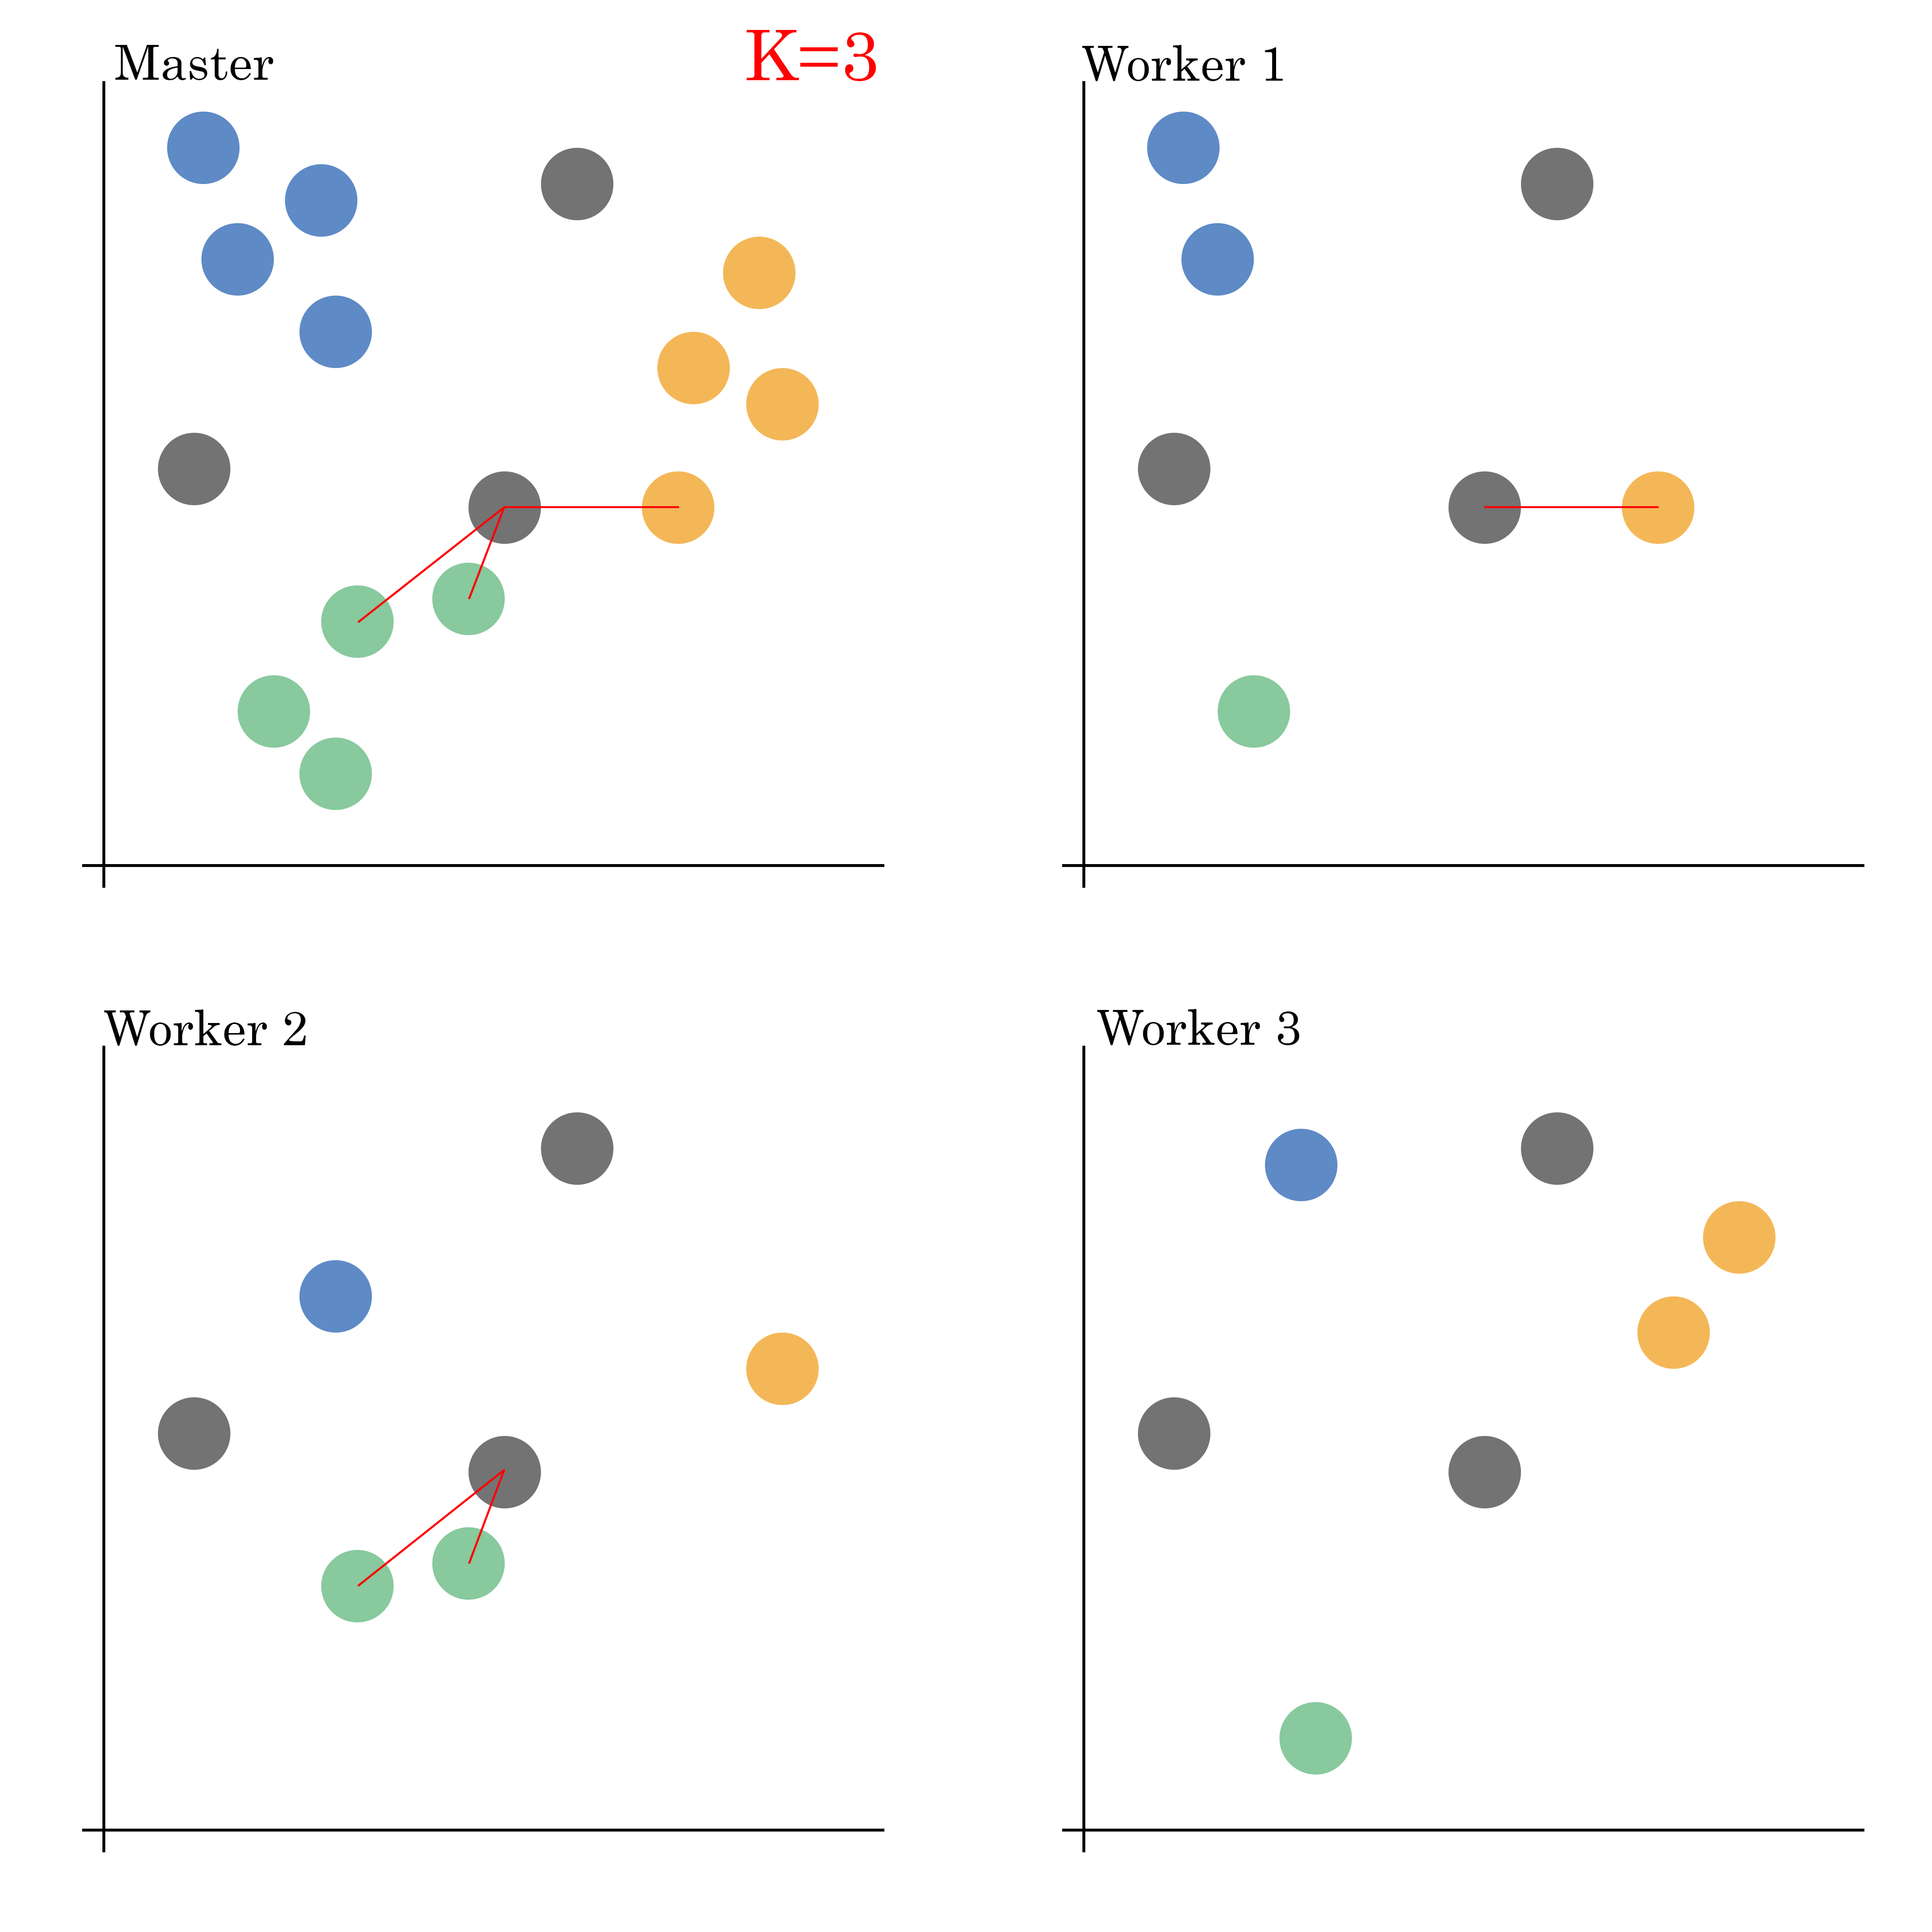
\includegraphics[width=\textwidth]{images/chapter_3/knn_mpi1}
				\caption{División de la población categorizada}
				\label{fig:knn1}
			\end{subfigure}
			\hfill
			\begin{subfigure}[t]{0.45\textwidth}
				\centering
				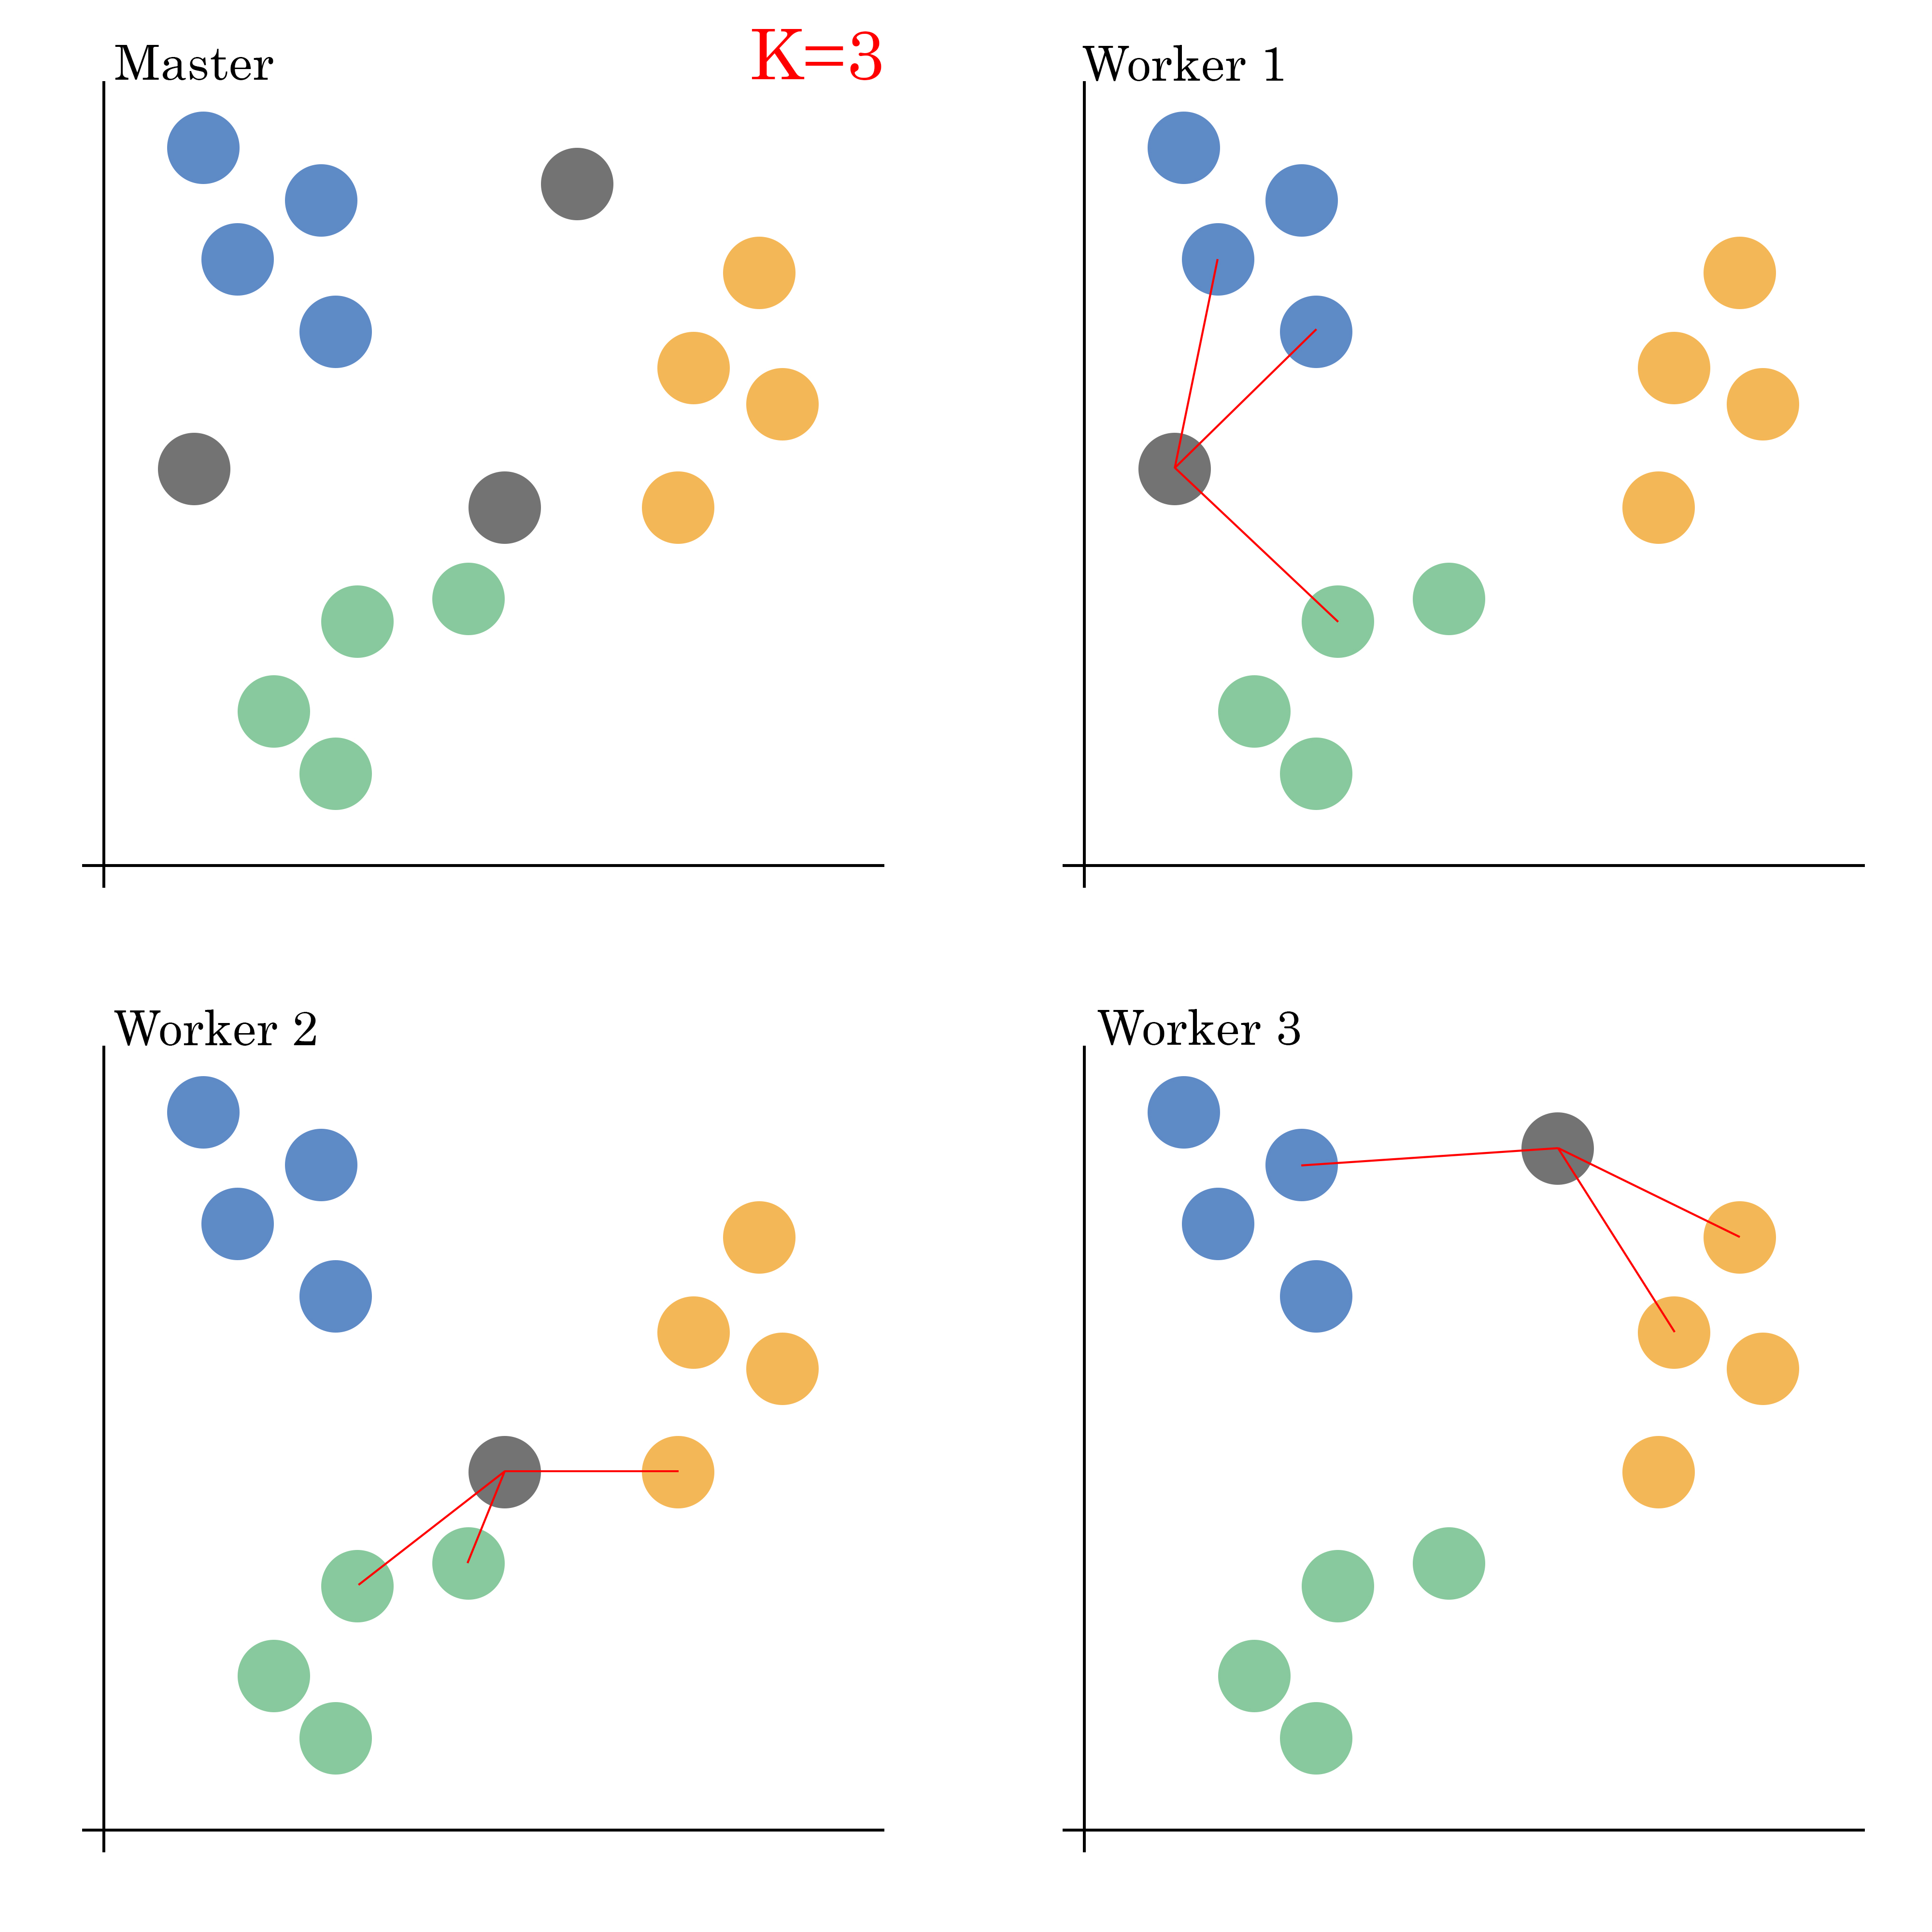
\includegraphics[width=\textwidth]{images/chapter_3/knn_mpi2}
				\caption{División de la población a predecir}
				\label{fig:knn2}
			\end{subfigure}
			
			\caption{MPI - Estrategias para paralelizar el algoritmo KNN}
			\label{fig:knnmpi}
		\end{figure}

		El proceso \textit{master} (el de la esquina superior izquierda en ambas figuras) tiene el dataset completo. En la primera estrategia (gráfico de la izquierda) divide la población categorizada (individuos representados con colores) entre los procesos y mantiene una copia en todos los procesos de la población a predecir (individuos representados en gris). La segunda estrategia (gráfico de la derecha) tiene una copia de la población categorizada en todos los procesos y una subpoblación de la población a predecir.
		
		
		En este algoritmo también hay que realizar una búsqueda del mejor valor para \textit{K}. Sin embargo, al contrario que en K-Medias, no hace falta repetir varias veces el mismo algoritmo, ya que el proceso es determinista. Es decir, con la misma población, siempre se obtiene la misma predicción. Aunque puede llegar a cambiar dependiendo del orden de categorización de la población a predecir. 
		
		No hay que repetir el mismo algoritmo varias veces, pero puede llegar a ser útil variar el número de vecinos (valor de \textit{K}). Las mejoras de esta búsqueda son las mismas que en el algoritmo anterior: 
		
		\begin{enumerate}
			\item Aplicar alguna de las dos implementaciones comentadas anteriormente, con un bucle que varíe la variable \textit{K}. 
			\item Ejecutar en cada proceso \textit{worker} el algoritmo sin mejoras. El \textit{master} se encarga de almacenar los mejores resultados.
		\end{enumerate}
		
		


\section{Aprendizaje por refuerzo}

	Los algoritmos de este tipo de aprendizaje actualizan iterativamente las estimaciones de calidad de las acciones permitidas en el entorno de desarrollo. 
	
	\subsection{Q-Learning}
		
		El algoritmo Q-Learning, es el más básico del aprendizaje por refuerzo. Las estimaciones de las mejores acciones para cada estado se almacenan en una Q-Table representada como una matriz en la que cada fila es un estado, y las columnas son las acciones disponibles. 
		
		Este algoritmo tiene numerosas aplicaciones. Nos centramos en la técnica de minimizar las acciones, para llegar desde una celda origen a un destino. El laberinto tiene un tamaño y semilla variable por parámetros de inicialización. Para lograr su objetivo dispone de acciones de movimiento en los dos ejes cardinales, norte, sur, este y oeste. No puede atravesar ni situarse en un muro del laberinto, y para que el agente aprenda a moverse por el laberinto y llegar a la meta hay que fijar unas recompensas:
		\begin{itemize}
			\item Si se choca con un muro castigamos al agente con valores altos para que no añada movimientos innecesarios para alcanzar su objetivo.
			\vspace*{-0.2cm}
			\item Al moverse, el agente recibe un castigo pequeño para que aprenda a minimizar las operaciones.
			\vspace*{-0.2cm}
			\item Al llegar a la meta le damos una recompensa alta, para que aprenda a la celda destino. 		
			\vspace*{-0.2cm}
		\end{itemize}
	
		Con estas recompensas, el agente aprende a llegar a la meta minimizando las acciones ejecutadas. El código que genera los laberintos ha sido implementado por @ChlouisPy en github\cite{MazeGenerator}


		Antes de enfocarnos en las implementaciones MPI, hay que comentar una mejora que se puede aplicar a el algoritmo básico de Q-Learning. Realizar un preprocesado. Modificar la Q-Table, convertiéndola en un array bidimensional, en el cual no se almacenen las acciones que no deseamos que realice el agente, como puede ser chocarse con un muro. O eliminar estados innacesibles como situarse en un muro.
		
		Esta mejora puede reducir el tiempo de cómputo, al no perder tiempo realizando acciones innecesarias para alcanzar su objetivo. Además de reducir la complejidad espacial, al reducir el número de estados. Un desventaja es que añade otras estructura adicional (array bidimensional) para almacenar las acciones para cada estado. 
		
		Este preprocesado tiene complejidad cuadrática \textit{O(4*N\(^{2}\)) $\equiv$ O(N\(^{2}\))}. Recorre toda la matriz, comprobando para cada celda si no es un muro, y en caso afirmativo itera en las cuatro direcciones permitidas para almacenar las acciones disponibles para la celda actual (estado). Con tamaños de laberintos pequeños no hace falta paralelizar el preprocesado, porque no se consigue reducir el tiempo significativamente. Laberintos con más de mil filas y columnas si se consigue reducir el tiempo de cómputo.
		
		
			
		En los algoritmos del bloque anterior se necesitaba realizar una búsqueda para encontrar el óptimo general. En este algoritmo conviene realizar otra búsqueda, pero esta vez para encontrar combinaciones de los hiper-parámetros ($\alpha$, $\gamma$, $\epsilon$). Son muy importantes para el desarrollo del agente en el entorno. Una mala configuración de éstos hace que sobre aprenda -o no aprenda- correctamente, generando bucles infinitos. Por este motivo es importante comprobar las diferentes combinaciones de hiper parámetros, y comprobar, cuales funcionan correctamente en el entorno. La búsqueda en laberintos grandes es muy lenta, ya que hay que comprobar muchas combinaciones entre los hiper-parámetros y los episodios del entrenamiento. Por eso es más útil desarrollar el algoritmo Deep Q-Learning que no tiene problemas con los estados, al usar una red neuronal. Pero si queremos usar el algoritmo básico de Q-Learning, hay que realizar una búsqueda exhaustiva en el entorno ejecutando una cantidad significativa de combinaciones de hiper parámetros.

		Para paralelizar esta búsqueda se ejecuta el algoritmo básico con el preprocesado mencionado en cada proceso \textit{worker}. Hay que desarrollar una estrategia para que cada \textit{worker} reciba una combinación de parámetros distinta, y así no haya repeticiones, perdiendo tiempo de cómputo. 
			
		El \textit{master} se encarga de repartir combinaciones de hiper-parámetros. Con una precisión previamente inicializada, el \textit{master} aumenta un hiper-parámetro hasta llegar al \textit{100\%}. Cuando llega a dicho límite, se reinicia la variable y se aumenta la siguiente. Este proceso continua hasta llegar al \textit{100\%} de todos los hiper-parámetros. Cada \textit{worker} se encarga de una combinación recibida. Cuando termina el algoritmo, ya sea por bucle infinito o finalización correcta, envía un mensaje al \textit{master} con la información de finalización y los hiper-parámetros usados.
		
		Si el mensaje de finalización indica ``bucle'', el proceso ha terminado para evitar que se convierta en un proceso inactivo, pues dicha conbinación no converge hacia el objetivo. Estos bucles se detectan en el entrenamiento o la evaluación. Hay un bucle en el entrenamiento si un episodio tarda más de \textit{X} segundos en finalizar. En la evaluación se comprueba teniendo en cuenta los últimos cuatro estados visitados. Pues avanza y retrocede constantemente. 
		\begin{center}
			\textit{Estados[0]==Estados[2] and Estados[1]==Estados[3] and Estados[0]!=Estados[1]: }
		\end{center}
		
		

		Una vez realizada una búsqueda de las combinaciones de hiperparámetros eficaces, se pueden emplearse para las siguientes mejoreas:
		
		\begin{enumerate}
			\item Dividir el entorno entre los procesos.
			\item Ejecutar el algoritmo en los \textit{workers} y juntar las experiencias.
		\end{enumerate}

	
		
		Al dividir el laberinto entre los procesos (primera mejora), cada proceso controla una zona, y se genera un flujo constante de episodios (iteraciones del algoritmo). Cuando un agente sale del dominio de un proceso, este le manda un mensaje al proceso que controla esa parte del laberinto con la posición en la que entra. La Figura \ref{fig:rlmpi} muestra como se divide un posible laberinto entre los procesos. Además de mostrar tres episodios con sus respectivos agentes (circulo en rojo). El \textit{master} se encarga de iniciar a los agentes en la celda en verde y cuando sale de su dominio envia al respectivo proceso y genera otro agente. 
		
		Para garantizar el correcto funcionamiento, el \textit{master} no puede recibir agentes de los \textit{workers}, en caso contrario no se podría garantizar el flujo de nuevos episodios. Solo puede existir \textit{M} agentes en todos los procesos (siendo \textit{M} el número de procesos ejecutados), debido a que un proceso solo puede gestionar a lo sumo un agente. 
		
		Cada proceso tiene su propio dominio, lo que provoca que la Q-Table se divide entre éstos. Aplicando el preprocesado comentado anteriormente se dividen los dos arrays bidimensionales (acciones y Q-valores). 
		
		
		
		\begin{figure}[!h]
			\centering
			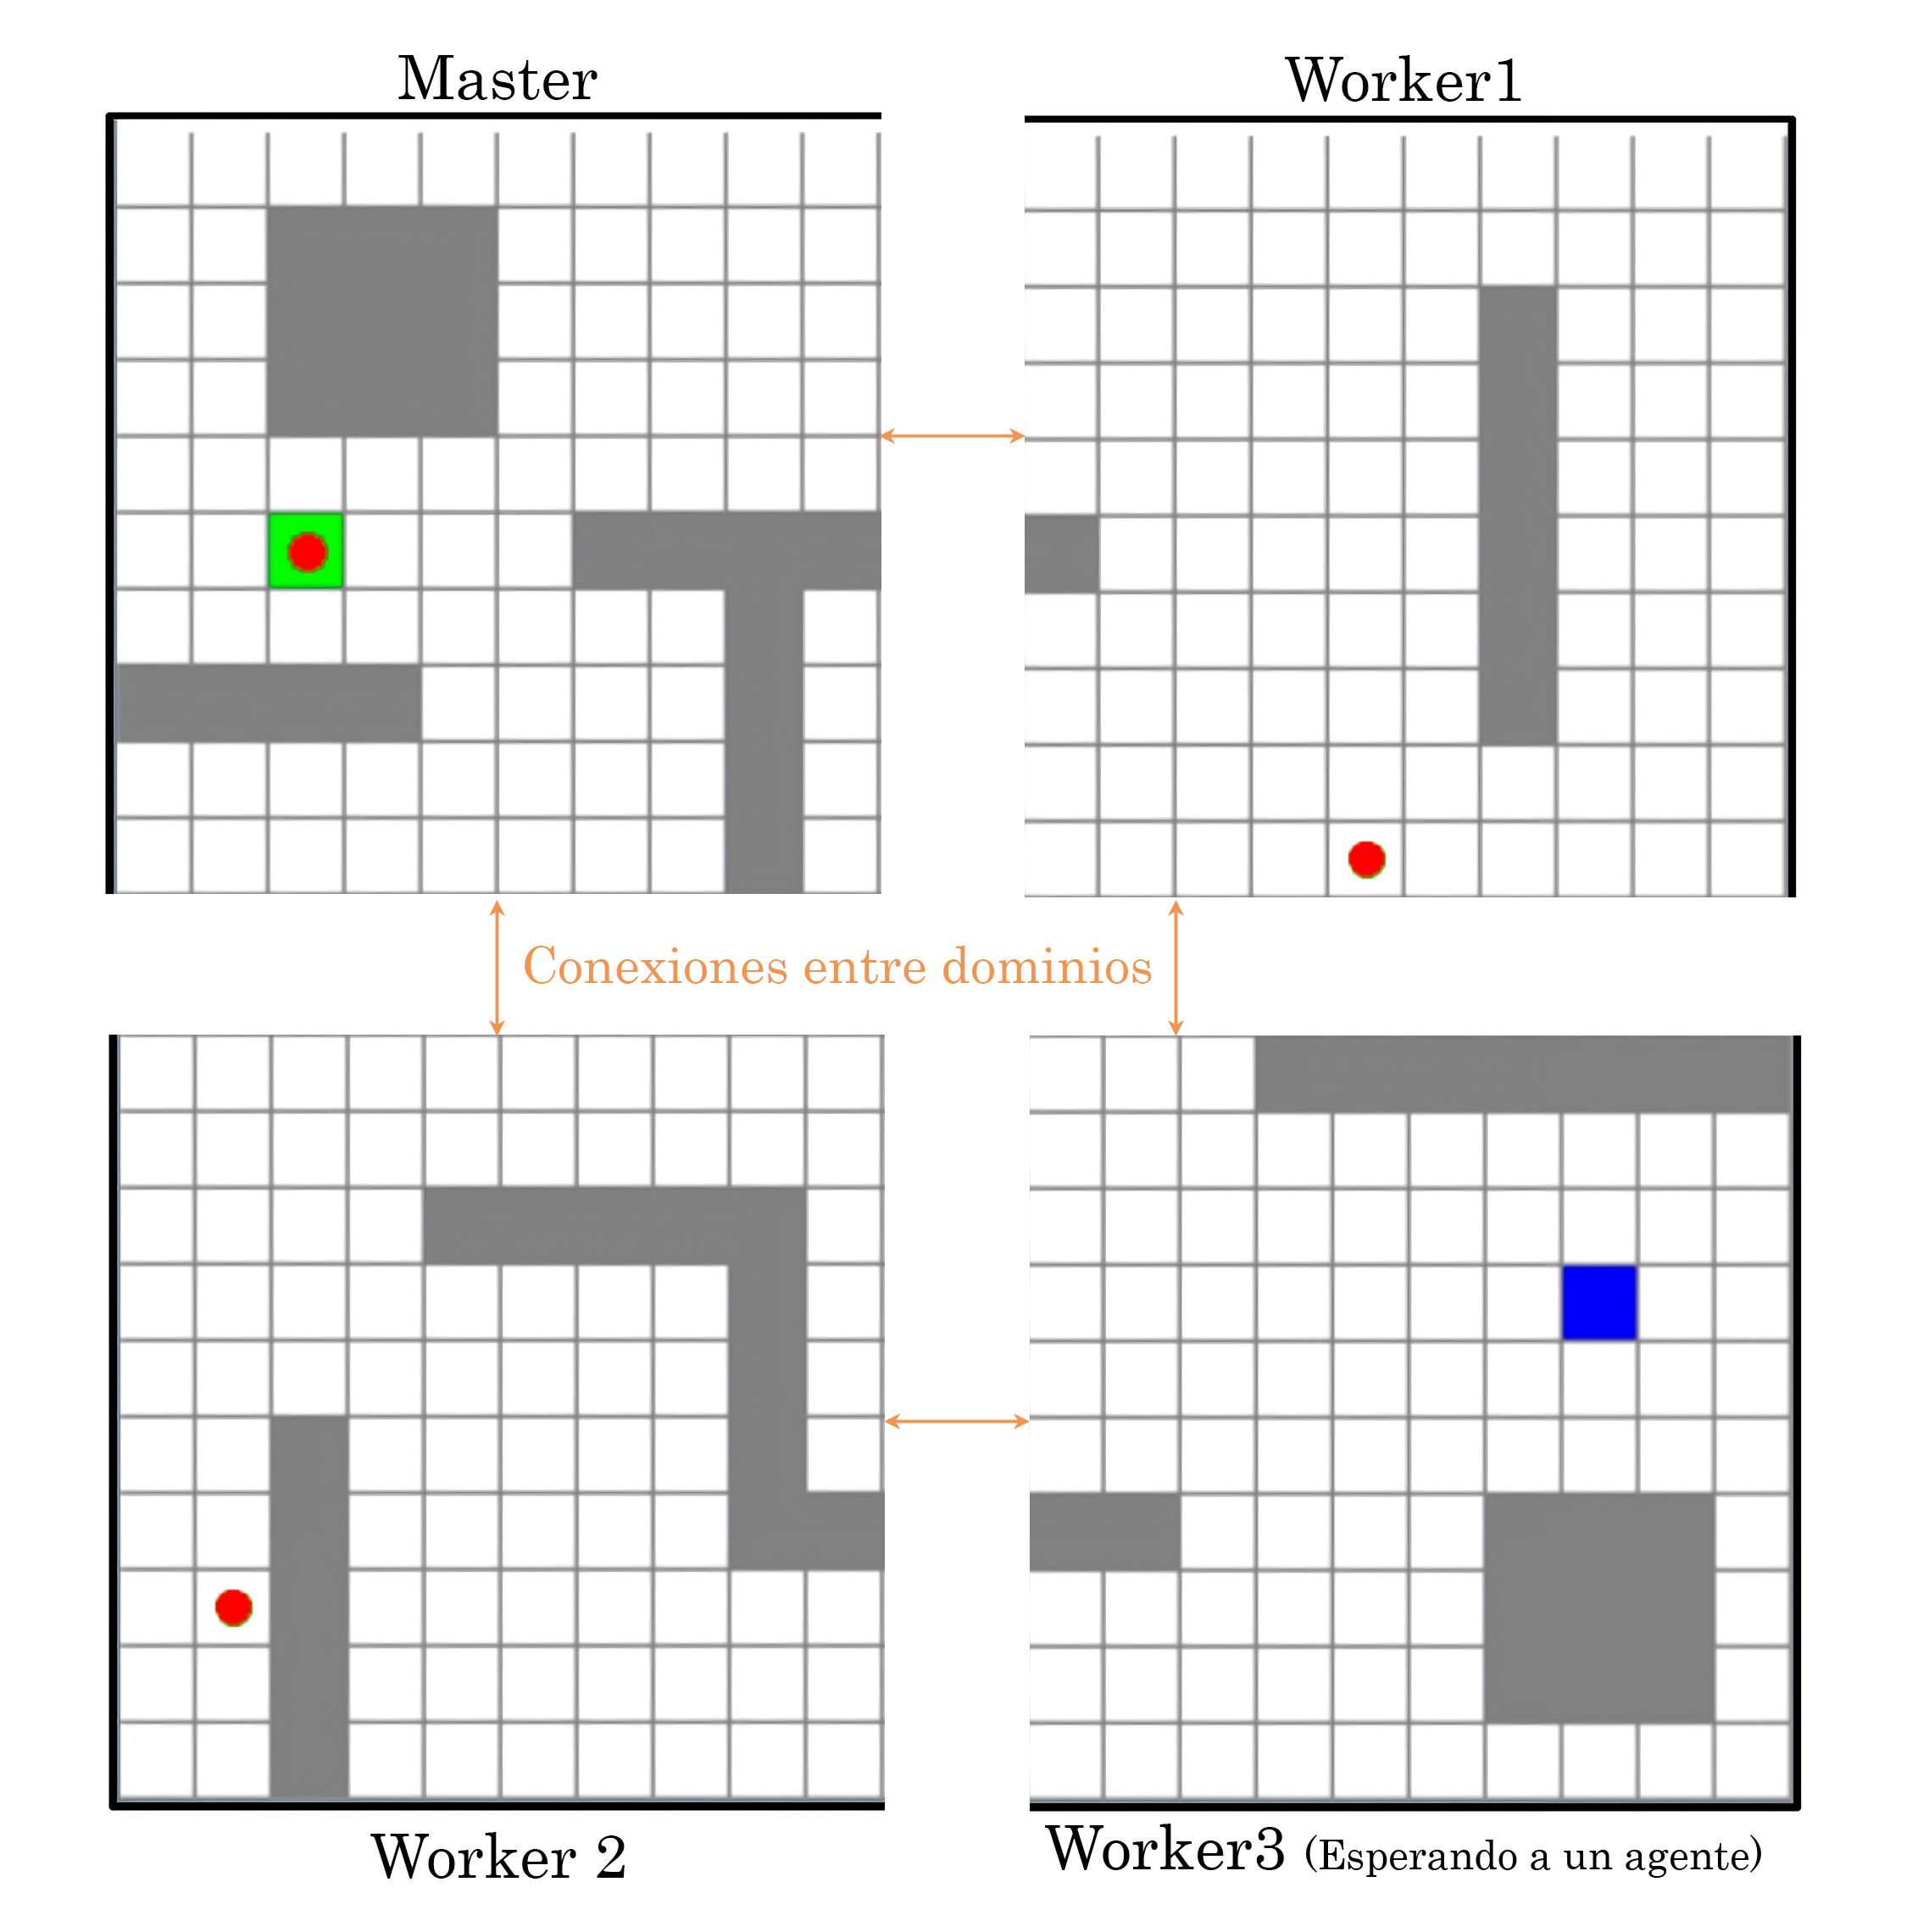
\includegraphics[width=0.6\textwidth]{images/chapter_3/rl_mpi}	
			\caption{Aprendizaje por Refuerzo - División del entorno}
			\label{fig:rlmpi}
		\end{figure}
	
		Aplicando la estrategia realizada en la búsqueda de hiper-parámetros, se puede ejecutar en varios procesos el algoritmo. El \textit{master} recolecta las experiencias de los \textit{workers}, haciendo la media de los valor-Q obtenidos de los procesos, calculando así las mejores acciones para cada estado. 
		
		Si ejecutamos desde el mismo punto el algoritmo en cada \textit{worker} no se puede garantizar que funcione correctamente, pues puede ser que 
		
		
		Es mucho mejor inicializar el algoritmo desde distintos puntos, para así explorar todo el laberinto y encontrar el mejor camino en menos tiempo. Al menos un worker inicia desde el punto de inicio que se desea evaluar, pues de lo contrario no se podría garantizar que visiten la zona del inicio, y obtengan las estimaciones correctas para llegar al destino.
			
			
	
	
	
	
	\subsection{DQN}
	
		Este algoritmo utiliza redes neuronales para obtener la mejor acción para un determinado estado, así eliminando los problemas que tiene el algoritmo anterior. Con es método podemos abarcar entornos más complejos, y por eso se propone el juego de atari Pac-Man, centrándonos en obtener el mayor número de monedas antes de provocar una condición de finalización. Antes de profundizar en el algoritmo de IA, explicamos el entorno del problema a resolver:
		\vspace{-0.5cm}
		\begin{itemize}		
			\item Acciones disponibles. Como en el algoritmo anterior, son de movimiento. El agente y los fantasmas no pueden atravesar muros.
			\vspace*{-0.2cm}
			\item Entorno. Laberinto con muros, del cual no se puede escapar.
			\item Objetos del juego. 
			\vspace*{-0.3cm}
				\subitem Pac-Man, el agente que mueve el usuario. Su objetivo es comer todos los puntos.
				\vspace*{-0.3cm}
				\subitem Fantasmas, se mueven siguiendo unos objetivos en el laberinto.
				\vspace*{-0.3cm}
				\subitem Túneles. Puntos que se conectan de manera toroidal para no salir del
				\vspace*{-0.3cm}
				\subitem Puntos (pellets en ingles). Son las "monedas" que el agente tiene que recoger.
				\vspace*{-0.3cm}
				\subitem Puntos de energia (powers). Si el agente consume uno, durante un periodo de tiempo es invencible y puede comer a los fantasmas.
				
				 laberinto.				
			\vspace*{-0.3cm}
			\item Condiciones de finalización. Ganar obteniendo todas las monedas del laberinto o perder si un fantasma come al agente. 			
		\end{itemize}
		
		\begin{flushleft}
			Los fantasmas tienen una IA interesante, pues tienen sus propios estados y cada uno tiene unos puntos objetivos que siguen para intentar comer al agente. Los estados son los siguientes:
		\end{flushleft}
		\vspace{-0.9cm}
		\begin{itemize}
			\item Chase. Cada fantasma sigue unos puntos en movimiento.
			\vspace*{-0.3cm}
			\item Scatter. Sigue un punto estático fuera del laberinto para dar vueltas en una determinada zona.
			\vspace*{-0.3cm}
			\item Frightened. El agente puede comerlos, se mueve de manera aleatoria al llegar a una intersección.
			\vspace*{-0.3cm}
			\item Eaten. Han sido comidos y se encuentran en su casa esperando a salir. (Implementado de forma que espera 3 movimientos del agente para salir)
		\end{itemize} 
		
		\begin{flushleft}
			En la estado \textit{Chase} los fantasmas se mueven de la siguiente forma:
		\end{flushleft}
		
		\vspace{-0.9cm}
		\begin{itemize}
			\item Blinky (Rojo): Persigue directamente al agente.
			\vspace*{-0.3cm}
			\item Pinky (Rosa): Persigue la celda cuatro posiciones adelantada a donde apunta el agente. Si el agente mira hacia arriba, también añade cuatro celdas hacia la izquierda
			\vspace*{-0.3cm}
			\item Inky (Azul): Persigue una celda en concreto que se calcula de la siguiente forma. Primero se calcula una posición como lo hace el fantasma rosa pero en vez de cuatro celdas, se hace con dos. El objetivo se calcula al añadir el vector de distancia de la posición del fantasma rojo a esta posición.
			\vspace*{-0.3cm}
			\item Clyde (Naranja): Si está a ocho o más celdas de distancia del agente, lo persigue. En caso contrario sigue su objetivo del estado Scatter.
		\end{itemize}
		
		El laberinto y el juego han sido creados desde cero para facilitar el aprendizaje del la IA, con estados mas sencillos y poder hacer los cambios necesarios en un futuro. El laberinto se almacena en un fichero de texto, para representar las celdas vacias, muros, puntos o puntos de poder con números enteros (0, 1, 2 y 3 respectivamente).
		
		
		
		
		\subsubsection{Entrenamiento}
			
			La fase de entrenamiento es crucial, pues modifican los valores de la red neuronal para que tome las mejores decisiones en cada estado, haciendo que el agente pueda terminar el problema sin perder.	El entrenamiento se puede realizar de varias formas.	
			
							
			Si mantenemos el mismo estado inicial, el agente empieza siempre en el mismo punto, y depende mucho de los hiperparámetros, además de la aleatoriedad. El agente empieza a investigar el entorno de manera aleatoria, y es muy probable que los fantasmas alcancen al agente bastante rápido sin explorar mucho el entorno. Por eso es mejor añadir varios estados iniciales para que pueda investigar el entorno de manera más eficiente. Hay que tener en cuenta que los estados iniciales tienen que ser puntos accesibles desde el estado inicial original. El agente no puede saltar a otros puntos sin coger los puntos del laberinto (Figura \ref{fig:pacman_states}), si entrenamos con puntos aleatorios sin cambiar el estado del laberinto, al ejecutar el algoritmo con los mejores valores obtenidos, no habrá servido de nada, pues son estados que el agente no va a alcanzar nunca.
			
		
			\begin{figure}[!h]
				\centering
				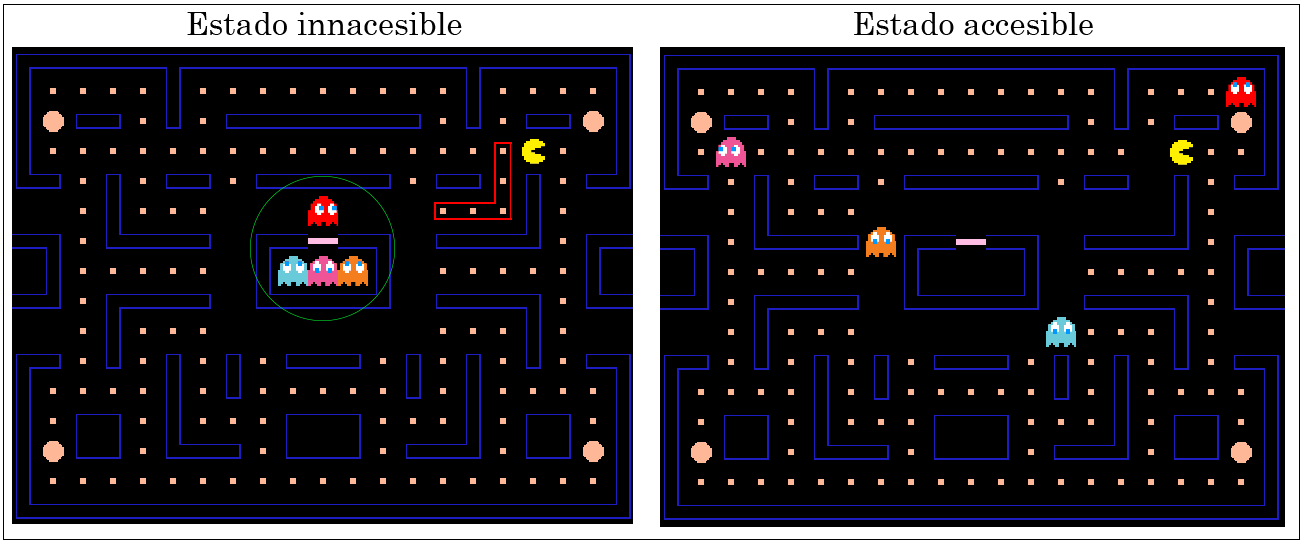
\includegraphics[width=1\textwidth]{images/chapter_3/pacman_states}	
				\caption{DQN - Estados del entorno}
				\label{fig:pacman_states}
			\end{figure}
			
			En la ejecución de la izquierda, el agente empieza en una posición aleatoria, sin cambiar los objetos del entorno. Este estado nunca se va a ejecutar, pues necesita coger los puntos del camino y cambiar las posiciones de los fantasmas, como se puede ver en la ejecución de la derecha.
			
		\subsubsection{Mejoras MPI}
		
			Al usar redes neuronales, se pueden aplicar las mejoras que se van a comentar en la sección de redes neuronales \ref{sec:redes_neu}. No se pueden aplicar las mejoras del algoritmo anterior, pues no es una matriz que se pueda dividir el trabajo, es una red neuronal cuyos pesos varían al ejecutar acciones en estados.
		
			
		
		
		
			
		
		
	
		
	
	\newpage
	


\section{Algoritmos Evolutivos}
	Los algoritmos evolutivos son sencillos de paralelizar, debido a que son procesos que se repiten muchas veces, y se ejecutan en muchos individuos.
	
	\begin{enumerate}
		\item \textbf{Inicialización.} Dados los parámetros iniciales se crea la población, con los individuos deseados. Hay diferentes tipos, con sus respectivas características.
		\begin{itemize}
			\item Binarios. Estos individuos son fáciles de inicializar, pero ralentizan la comunicación entre procesos, debido a tener que enviar muchos bits.
			\item Reales. Parecidos a los binarios pero estos son más portables.
			\item Árboles. Más lentos para inicializar y difíciles de tratar.
		\end{itemize}
		
		\item \textbf{Evaluación.} Este es el método que más tiempo de ejecución puede llegar a consumir. Varía dependiendo del tipo de individuo del problema.
		
		\item \textbf{Selección.} Se seleccionan a los individuos. El tiempo depende de los métodos de selección aplicados, pero suelen ser lineales.
		
		\item \textbf{Cruce.} Con una cierta probabilidad, se cruzan 2 individuos del conjunto seleccionado. Tienen un mayor coste que selección.
		
		\item \textbf{Mutación.} Igual que el cruce tiene una probabilidad para mutar. Parecido a cruce, pero un poco más rápido.
	\end{enumerate}
	
	Para cada tipo de individuos se desarrollan unos problemas.\\
	1. Binario, con un intervalo dado y una precisión, queremos calcular el valor máximo o mínimo para ciertas funciones. Los valores fitness se calculan con la representación real del cromosoma, que varía dependiendo de la precisión que se le asigna al ejecutar el algoritmo. Por lo que hay que convertir de binario a real.
	Este problema se ejecuta bastante rápido. Reducir su tiempo de ejecución es desafiante.\\
	2. Real. Aeropuertos con un número variable de vuelos y pistas. Queremos calcular el sumatorio de tiempos mínimos de retraso para que los aviones aterricen en el aeropuerto. Cada avión tiene asignada la hora de aterrizaje para cada pista, y hay un tiempo mínimo de separación entre vuelos que aterrizan en cada pista. Se puede resolver con vuelta atrás pero tiene un coste exponencial (inviable). El valor fitness tiene coste \textit{O(NumAviones*NumPistas) $\equiv$ O(\(N^{2}\))}. Se calcula:
	
	\lstset{language=python, 
		breaklines=true, 
		basicstyle=\footnotesize,
		backgroundcolor=\color{lightergray},
		commentstyle=\color{green_comment},}
	\begin{lstlisting}
 fitness=0
 for avion in aviones:
 for pista in range(pistas): # Calculamos TLA para cada pista
 TLA = maximo(TLA(vuelo_anterior) + SEP[vuelo_anterior][vuelo_actual], TEL)
 # Se asigna el vuelo actual a la pista con minimo TLA calculado
 fitness+=(menor_TLA-menor_TEL)^2
 # menor_TEL: menor TEL de ese vuelo con todas las pistas		
	\end{lstlisting}
	
	\noindent El tiempo de ejecución para este problema depende de la función de evaluación, que varía dependiendo del número de aviones y pistas. 
	
	3. Árbol, tenemos una matriz de enteros que representa un jardín. 1: césped y                 0: césped podado. Queremos maximizar el área podada. Para ello el agente tiene unas acciones que puede ejecutar.
	El coste temporal de este algoritmo viene dado principalmente por la función de evaluación. Ejecuta la simulación en la matriz hasta cumplir un determinado número de ticks (acciones realizadas), que es proporcional al número de filas y columnas de la matriz. Aunque las funciones de cruce y mutación también tardan en ejecutarse, debido al control de punteros.
	
	
	
	\begin{flushleft}
		Cada una de las siguientes mejoras MPI se pueden configurar para cada tipo de individuo.\\
		1. Dividir la población en subpoblaciones.\\
		2. Modelo de islas.\\
		3. PipeLine. (Figura \ref{fig:pevpipe})\\
	\end{flushleft}
	
	La primera implementación, de dividir la poblacion entre procesos, se puede paralelizar fácilmente. El master recibe de los Workers las subpoblaciones inicializadas y evaluadas, y comienza el bucle principal del algoritmo, en el cual:
	\begin{itemize}
		\item El master se encarga de hacer la selección, y enviarla dividida a los workers. Mientras los workers trabajan, el master almacena el progreso de los mejores individuos de cada generación.
		\item Los workers reciben la selección, la cruzan, mutan y evalúan. Al finalizar estos procesos mandan la subpoblación al master para empezar la siguiente iteración.
	\end{itemize}
	
	Para el \textbf{modelo de islas}, se aplica la idea de mejoras pasadas, en cada proceso se ejecuta el algoritmo. Todos tienen el mismo tamaño, pero distintas poblaciones. Hay varios tipos de comunicaciones en esta mejora. Cada cierto tiempo se reinicia la población con los mejores individuos generales (de todos los procesos).

	\begin{itemize}
		\item Estrella. Solo hay comunicaciones master-worker. El master recibe los mejores individuos.
		\item En red. No hay proceso master, todos los procesos ejecutan el algoritmo. Todos los procesos están en comunicación constante, mandando los mejores individuos para el reinicio de la población.
		\item En anillo. Tampoco hay proceso master, los procesos se comunican como una lista enlazada.
	\end{itemize}
	
	Segmentar el algoritmo entre los procesos, provoca un flujo constante de generaciones. Cada proceso se encarga de un método. El master se encarga de generar cuatro poblaciones distintas y las evalúa para mandarlas al worker que se encarga de la selección. El master no genera más poblaciones, y pasa a un estado de recepción mejores individuos. Las poblaciones van evolucionando conforme avanzan por el pipeline. El último worker se encarga de la evaluación, que envía al worker de selección, y al master.
	
	\begin{figure}[!h]
		\centering
		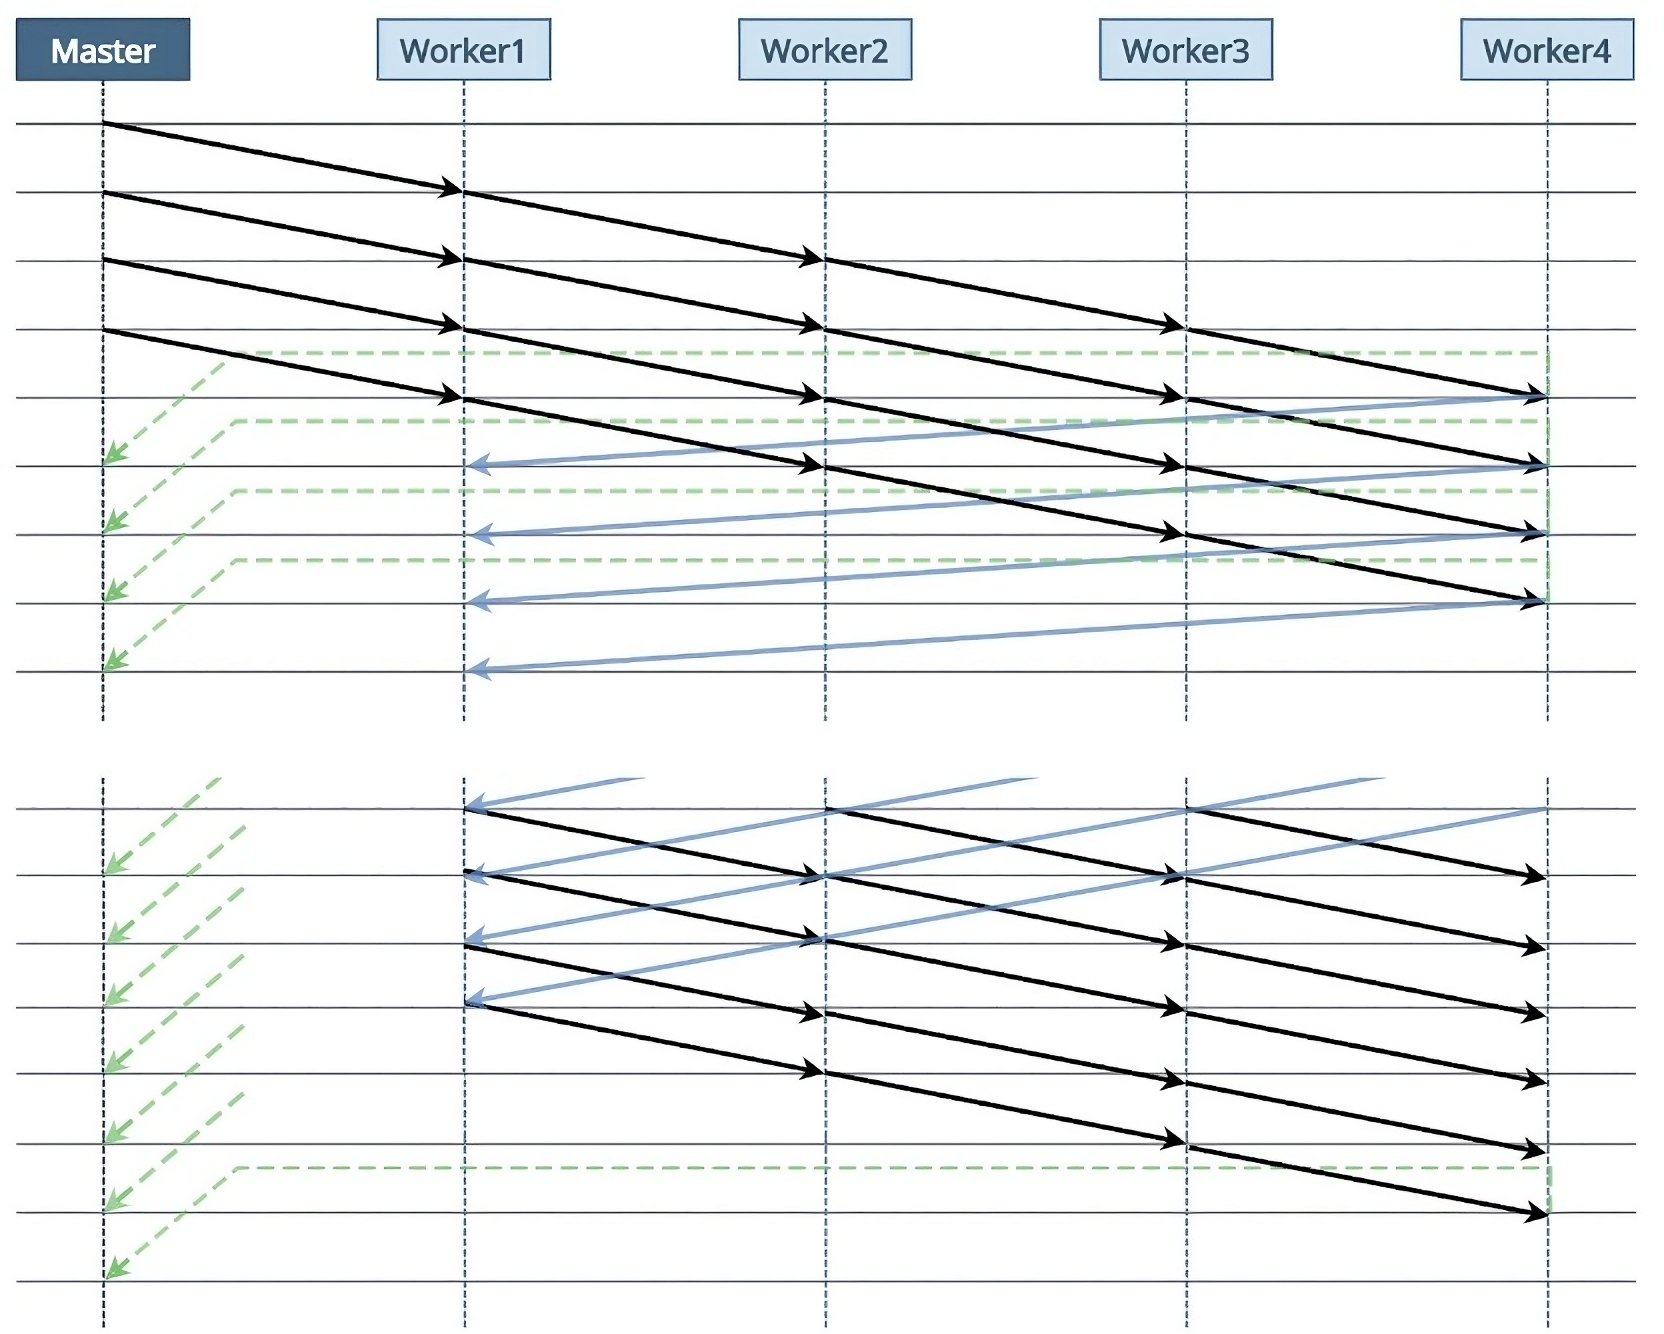
\includegraphics[width=0.65\textwidth]{images/chapter_3/pev_mpi3}
		\caption{MPI - PEV PipeLine}
		\label{fig:pevpipe}
	\end{figure}

	Se puede reducir el tiempo de ejecución si comprobamos que métodos tardan más, añadiendo más procesos para reducir la carga de trabajo.
	
	
	
	
	


\section{Redes Neuronales}
\label{sec:redes_neu}	
	Esta poderosa herramienta de aprendizaje supervisado, está diseñada para reconocer patrones complejos y realizar diversas tareas. Aprende con un proceso iterativo de entrenamiento, ajustando las conexiones entre neuronas. Este proceso secuencial es complejo de paralelizar. Al finalizar una predicción el modelo se tiene que actualizar propagando hacia atrás.
	
	Nos centramos en la técnica de \textbf{predicción}. La capa de entrada está formada por dos neuronas, cada individuo son variables numéricas que representan, la altura y el peso de una persona, y aprende a predecir el Índice de Masa Corporal (IMC). La capa de entrada y salida no varían, pero la capa oculta se puede modificar libremente, aumentando el tiempo en la fase de entrenamiento.
	
	
	Como en algoritmos pasados, necesitamos encontrar la mejor tasa de aprendizaje, para que aprenda lo mejor posible. Por lo que diseñamos una programa MPI, en el cual se ejecutan en varios procesos el mismo algoritmo con diferentes tasas de aprendizaje y repeticiones para el entrenamiento. El speedup es proporcional al número de procesos.
	
	\begin{flushleft}
		Como en el algoritmo anterior, se puede aplicar un pipeline para que haya un flujo de mensajes, pero esta vez en vez de ser unidireccional es bidireccional, al tener que actualizar los pesos de las neuronas al predecir un individuo.\\	
		1. PipeLine\\
		2. Dividir el trabajo en procesos
	\end{flushleft}
	
	Segmentar el proceso de entrenamiento puede llegar a ser beneficioso. Cada proceso se encarga de una capa de la red neuronal, siendo el master el encargado de enviar individuos de la población categorizada. El último worker controla la capa de salida, con las etiquetas calcula el error y lo propaga hacia atrás. Para el correcto funcionamiento, hay que crear un buen diseño para tener un flujo constante de mensajes. Figura \ref{fig:redneumpipipe}.
	
	
	
	\begin{enumerate}
		\item El master envía un número proporcional de individuos al número de procesos ejecutándose. Luego entra en un bucle en el cual recibe el error, actualiza, y envía otro individuo. Para finalizar recibe el mismo número de individuos que envió al principio y actualiza.
		\item El último worker solo recibe las predicciones y calcula el error.
		\item Los workers de la capa oculta tienen un proceso más complejo. Primero reciben un número de individuos proporcional a su id, los procesan y envían. Después entran en un bucle en el cual:			
		\begin{itemize}
			\item Reciben, de la capa siguiente, los errores, actualizan sus pesos y envían a la capa anterior.			
			\item Reciben, de la capa anterior, los nuevos individuos, procesan y propagan hacia adelante.
		\end{itemize}		
		
	\end{enumerate}
	
	\begin{figure}[!h]
		\centering
		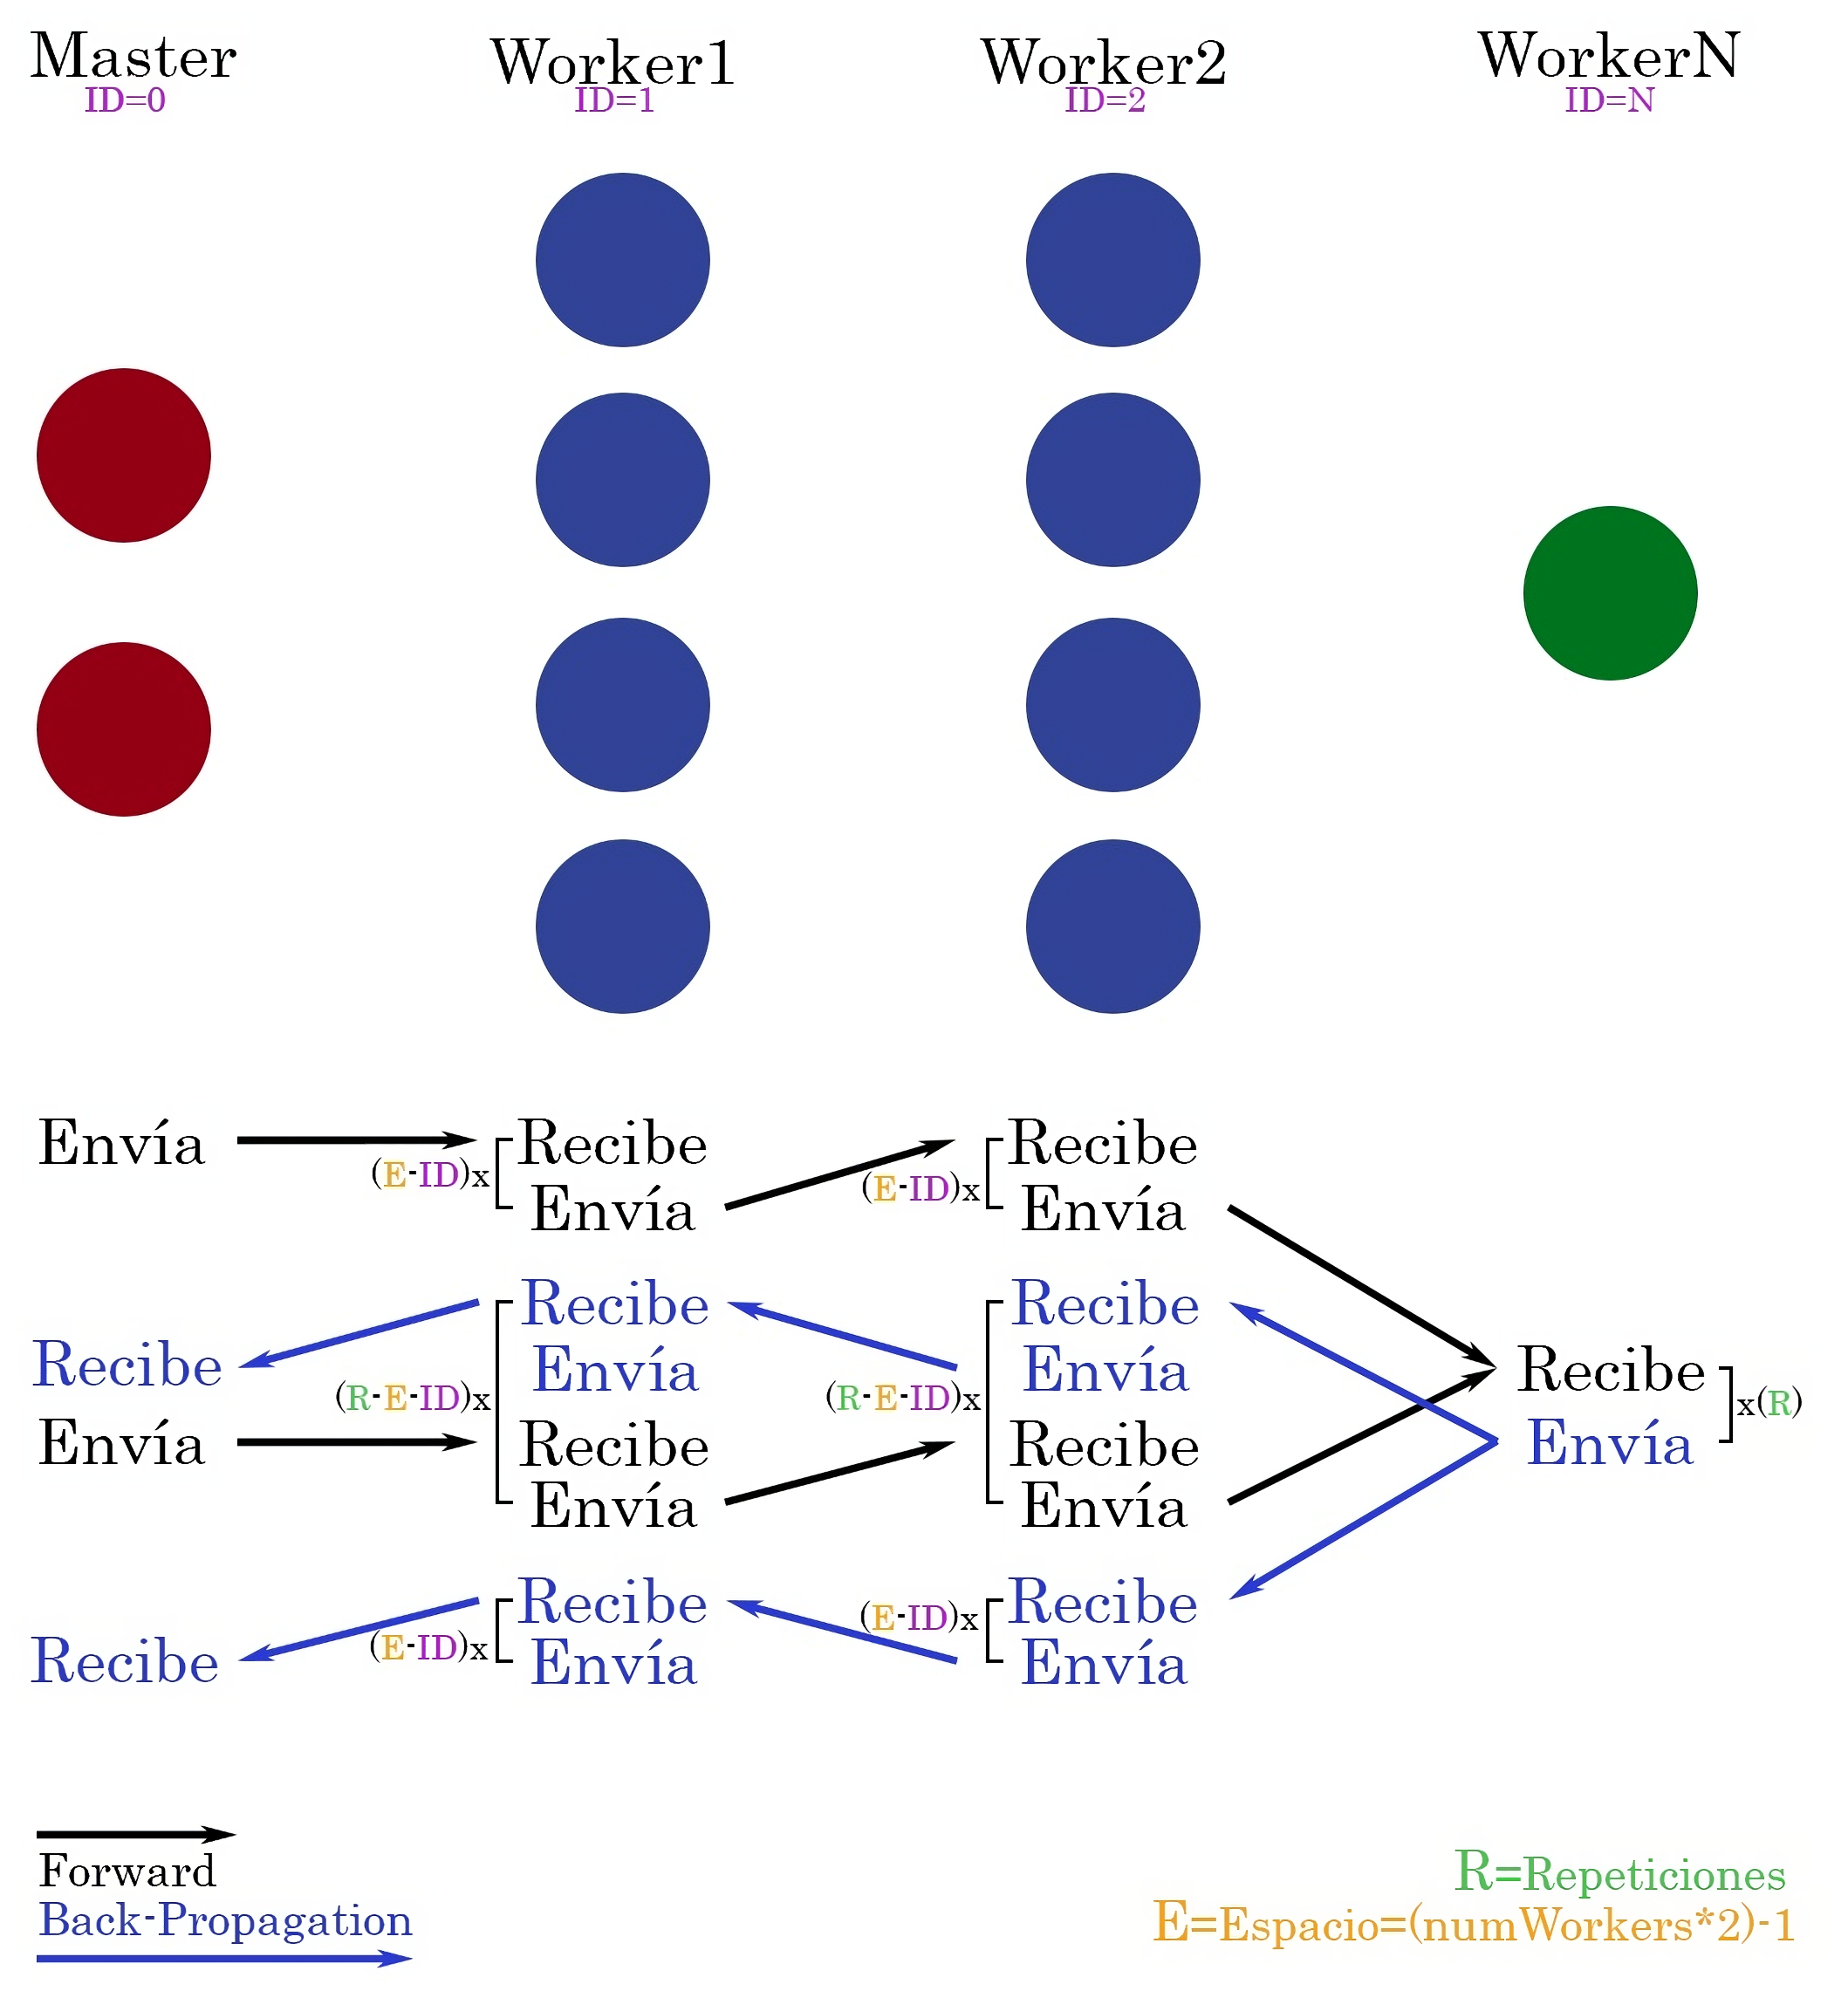
\includegraphics[width=0.55\textwidth]{images/chapter_3/redneu_mpi2}
		\caption{MPI - PipeLine Rede Neuronal}
		\label{fig:redneumpipipe}
	\end{figure}
	
	Al ser un proceso iterativo, en el cual el modelo va aprendiendo en la fase de entrenamiento, a primera vista, dividir la población entre procesos no parece ser beneficioso para el correcto aprendizaje de la red. Sin embargo, en redes neuronales hay un proceso llamado fine tuning \cite{malladi2023fine} que consiste en entrenar una red neuronal, con unos pesos ya calculados. Basándonos en esta técnica, podemos implementar una mejora en la cual dividamos la población inicial entre procesos, y en paralelo ejecutamos la fase de entrenamiento. Una vez finalizadas el master recibe los pesos de cada worker y hace la media. 
	
	Cuanto más grande sea la red neuronal mejor, tanto en rendimiento como en evaluación. En las redes neuronales grandes, un nodo se especializa en unos ciertos parámetros, por lo que no hay demasiadas intersecciones entre los entrenamientos de los procesos. Pero hay que dividir correctamente la población inicial entre los procesos. 
	
	\begin{enumerate}
		\item Con una población distinta, depende del tamaño de la red. 
		\begin{itemize}
			\item Si es una red pequeña, esta técnica no es muy efectiva. La diferencia de pesos entre procesos puede llegar a ser grande, y al hacer la media dar evaluaciones incorrectas. 		
			\item Sin embargo con muchas capas se mejora la evaluación. Cada proceso especializa unas neuronas y al juntarlas en el master no intersecan.			
		\end{itemize}		
		\item Si enviamos una población parecida, depende de la inicialización de los pesos, pero muy seguramente no surta efecto. Es como ejecutar varias veces el algoritmo en diferentes ejecuciones.
		
	\end{enumerate}	
	
	

	